%% 
%% Copyright 2007-2025 Elsevier Ltd
%% 
%% This file is part of the 'Elsarticle Bundle'.
%% ---------------------------------------------
%% 
%% It may be distributed under the conditions of the LaTeX Project Public
%% License, either version 1.3 of this license or (at your option) any
%% later version.  The latest version of this license is in
%%    http://www.latex-project.org/lppl.txt
%% and version 1.3 or later is part of all distributions of LaTeX
%% version 1999/12/01 or later.
%% 
%% The list of all files belonging to the 'Elsarticle Bundle' is
%% given in the file `manifest.txt'.
%% 
%% Template article for Elsevier's document class `elsarticle'
%% with harvard style bibliographic references

% \documentclass[preprint,12pt]{elsarticle}

%% Use the option review to obtain double line spacing
\documentclass[preprint,review,12pt]{elsarticle}

%% Use the options 1p,twocolumn; 3p; 3p,twocolumn; 5p; or 5p,twocolumn
%% for a journal layout:
%% \documentclass[final,1p,times]{elsarticle}
% \documentclass[final,1p,times,twocolumn]{elsarticle}
%% \documentclass[final,3p,times]{elsarticle}
%%\documentclass[final,4p,times,twocolumn]{elsarticle}
%% \documentclass[final,5p,times]{elsarticle}
% \documentclass[final,5p,times,twocolumn]{elsarticle}

%% For including figures, graphicx.sty has been loaded in
%% elsarticle.cls. If you prefer to use the old commands
%% please give \usepackage{epsfig}

%% The amssymb package provides various useful mathematical symbols

\usepackage{multirow}

\usepackage{tikz}
\usetikzlibrary{shapes.geometric, arrows.meta, positioning}

\tikzstyle{startstop} = [rectangle, rounded corners, minimum width=3cm, minimum height=1cm,text centered, draw=black, fill=blue!20]
\tikzstyle{process} = [rectangle, minimum width=3.5cm, minimum height=1cm, text centered, draw=black, fill=orange!30]
\tikzstyle{decision} = [diamond, aspect=2, minimum width=3cm, minimum height=1cm, text centered, draw=black, fill=green!30]
\tikzstyle{arrow} = [thick,->,>=stealth]


\usepackage{amssymb}

%% The amsmath package provides various useful equation environments.
\usepackage{amsmath}
%% hyperref must be loaded before cleveref; it also provides a catcode-safe
%% \url, needed by the URLs in the bibliography.
\usepackage[hidelinks]{hyperref}
\usepackage{cleveref}
\usepackage{stfloats}

\usepackage{float}
\usepackage{placeins}

\usepackage{xcolor}

%% Marking of the revised parts. Set \highlightfalse to obtain the clean version.
\definecolor{revtwo}{RGB}{0,90,200}
\definecolor{revthree}{RGB}{200,90,0}
\newif\ifhighlight
\highlighttrue
\newcommand{\rtwo}[1]{\ifhighlight\textcolor{revtwo}{#1}\else#1\fi}
\newcommand{\rthree}[1]{\ifhighlight\textcolor{revthree}{#1}\else#1\fi}
\newcommand{\rtwocolor}{\ifhighlight\color{revtwo}\fi}
\newcommand{\rthreecolor}{\ifhighlight\color{revthree}\fi}
\usepackage{soul}
%% The amsthm package provides extended theorem environments
%% \usepackage{amsthm}

%% The lineno packages adds line numbers. Start line numbering with
%% \begin{linenumbers}, end it with \end{linenumbers}. Or switch it on
%% for the whole article with \linenumbers.
\usepackage{lineno}

%\journal{Nuclear Physics B}

\begin{document}
\linenumbers

\begin{frontmatter}

%% Title, authors and addresses

%% use the tnoteref command within \title for footnotes;
%% use the tnotetext command for theassociated footnote;
%% use the fnref command within \author or \affiliation for footnotes;
%% use the fntext command for theassociated footnote;
%% use the corref command within \author for corresponding author footnotes;
%% use the cortext command for theassociated footnote;
%% use the ead command for the email address,
%% and the form \ead[url] for the home page:
% \title{Title\tnoteref{label1}}
%% \tnotetext[label1]{}
%% \author{Name\corref{cor1}\fnref{label2}}
%% \ead{email address}
%% \ead[url]{home page}
%% \fntext[label2]{}
%% \cortext[cor1]{}
%% \affiliation{organization={},
%%             addressline={},
%%             city={},
%%             postcode={},
%%             state={},
%%             country={}}
%% \fntext[label3]{}

\title{The Fission Matrix Method for Criticality Search in Heat-Pipe Micro Reactors} %% Article title

%% use optional labels to link authors explicitly to addresses:
\author[label1]{Christian Vita}
\author[label1]{Nicol\`o Abrate} %% Author name
\author[label1]{Sandra Dulla} %% Author name
\author[label5,label6]{Valerio Mascolino} %% Author name
\author[label3]{William Walters} %% Author name
\author[label2]{Nicolas Stauff}
\author[label4]{Fausto Franceschini}

\affiliation[label1]{organization={NEMO group, Energy Department, Politecnico di Torino},
            addressline={Corso Duca degli Abruzzi 24},
            city={Turin},
            postcode={10129},
            state={Italy},
            %country={}
            }

\affiliation[label2]{organization={Argonne National Laboratory },
            %addressline={},
            city={Lemont},
           % postcode={},
            state={IL},
            country={USA}}

\affiliation[label3]{organization={Westinghouse Electric Company},
            %addressline={},
            city={Cranberry},
            %postcode={},
            state={PA},
            country={USA}}
            
\affiliation[label4]{organization={Westinghouse Mangiarotti},
            addressline={v. Timavo 59},
            city={Monfalcone},
            postcode={34074},
            state={Italy},
            %country={}
            }

\affiliation[label5]{organization={Nuclear Science and Engineering},
            addressline={Colorado School of Mines},
            city={Golden},
            postcode={80401},
            state={CO},
            country={USA}}

\affiliation[label6]{organization={Department of Mechanical Engineering},
            addressline={Colorado School of Mines},
            city={Golden},
            postcode={80401},
            state={CO},
            country={USA}}


%% Abstract
\begin{abstract}
%% Text of abstract

% The Fission Matrix (FM) method provides the number of fission neutrons born in one core cell per fission neutrons in another cell. The method is applied to conduct the neutronics analysis of a Heat-Pipe Micro Reactor (HPMR). The aim of this model is to support the real-time modelling of heat-pipe-based microreactor designs, which have recently gained significant industrial interest.
In this work the Fission Matrix (FM) method is proposed to conduct the neutronics analysis of a Heat-Pipe Micro Reactor (HPMR). The aim of this model is to support the real-time modelling of heat-pipe-based microreactor designs, which have recently gained significant industrial interest. 

% A database of FMs is generated at various uniform temperatures and Control Drum (CD) rotation angles using the Monte Carlo code Serpent 2. This database is then used to interpolate FMs at intermediate conditions not explicitly included in the dataset. By solving the eigenvalue problem of the interpolated FM, the corresponding effective multiplication factor ($k_{eff}$) and fission source distribution ($F(\vec{r})$) are obtained.
A database of FMs is generated through different criticality calculations, each of them considering a different core configuration (temperature profile and control drums position). The database is then interpolated to generate, in principle, the results for any arbitrary core layout.

In this study the accuracy decrease of the FM method in the presence of a temperature difference between the core and the reflector is highlighted and addressed.    


% The accuracy of the method is assessed by comparison against reference Serpent 2 simulations. The analysis is conducted under various temperature distributions and CD positions. The study also highlights the negative impact on accuracy caused by large temperature differences between the core and the reflector. To address this, a correction ratio is defined, which requires only a relatively small number of additional FMs to be added to the database.

% The results generally show good agreement with the corresponding reference values. It has been demonstrated that, when a strong temperature gradient exists between the reflector and the core, the errors can increase significantly. However, thanks to the defined correction ratio, a very close agreement with the reference values is restored. Furthermore, the method has been tested under extremely strong (and unrealistic) temperature gradients within the core, and it still provides satisfactory results.

% Leveraging the computational efficiency and high accuracy of the FM approach, a custom criticality search algorithm is developed. The interpolated FMs are solved iteratively, updating the CD positions and the resulting temperature distribution until criticality is achieved ($k_{eff} = 1$).

% The accuracy of the criticality search algorithm is tested by considering four different cases, each varying the total power---and consequently the temperature distribution of the system---using a hypothetical correlation between the two variables. When applying the same CD angles obtained with Serpent 2 for the corresponding configurations, the results show a high degree of consistency with the reference.
The accuracy of the method is assessed through comparison with reference Serpent 2 simulations. Different core temperature profiles and control drum positions are tested. Finally, leveraging the computational efficiency and high accuracy of the FM, a criticality search algorithm is developed.

Overall, the results show very good agreement with the corresponding Serpent 2 reference cases, while requiring only a very short computational time.

\end{abstract}


%% Keywords
\begin{keyword}

Fission matrix \sep criticality search \sep heat-pipe micro reactor \sep HPMR

\end{keyword}


\end{frontmatter}

%% Add \usepackage{lineno} before \begin{document} and uncomment 
%% following line to enable line numbers
%% \linenumbers

%% main text
%%

%% Use \section commands to start a section
\section{Introduction} \label{section:Introduction}
%% Labels are used to cross-reference an item using \ref command.

Monte Carlo codes are regarded as one of the most accurate tools for neutronics calculations due to their continuous treatment for the angle and energy variables and to their capability of accurately modelling any complex geometry. Nevertheless, these simulations incur substantial computational expense when low statistical uncertainty is needed, especially in localized tallies. This computational burden makes the Monte Carlo method less practical for applications that require a large number of calculations, such as reactor modelling calculations including, e.g., transient simulations and criticality search.

To overcome this, alternative hybrid approaches were proposed, such as those based on the fission matrix (FM) method \cite{Carney2014}. The FM method requires the geometrical domain of the reactor to be subdivided into $N$ fissionable regions (or cells), used to tally the average number of neutrons generated in the \textit{i}-th cell due to fission reactions induced by a fission neutron born in the \textit{j}-th cell. This information is collected in the form of a $N \times N$ matrix ($\textbf{A}$), called the fission matrix. In multiplying systems, the fundamental eigenvector $F_0(\vec{r})$ of the fission matrix $\textbf{A}$ represents the fission source distribution, while its principal eigenvalue corresponds to the multiplication factor, $k_{eff}$.
The fission matrix method has been applied in various contexts, including full-core power reactor simulations \cite{Walters2018} and transient analyses \cite{Laureau2015}.
In this framework, the RAPID code represents an important implementation of the FM approach. Extensive validation of the RAPID code—both computational and experimental—has been carried out, given its foundation on the FM method \cite{RAU2020103273,Mascolino2022,Mascolino_trapid}.

This work presents an application of the FM method to model the Virtual Test BED Heat Pipe Micro Reactor (VTB-HPMR) design, described in the next section. The purpose is to demonstrate that the method can be applied also for this type of advanced reactor design, especially when the FM is parametrized with respect to 3D temperature distributions and control drums positions. After an assessment on the accuracy of the method, the paper presents a fast and accurate criticality search algorithm that could be applied for the real-time reactor monitoring. This computational framework could be particularly suited for the remote handling of microreactors.

\section{HPMR Model} \label{section:VTB HPMR model}
The model used in this work is based on the Micro-Reactor design under analysis at the Argonne National Laboratory (ANL) by the NEAMS Micro-Reactor Application Drivers area \cite{Stauff2024}. As a modelling exercise, the micro-reactor concept was designed at ANL to gather some of the most pressing modelling challenges faced by the micro-reactor industry, which are: the use of heat pipe technologies to remove the nuclear heat, the use of TRi-structural ISOtropic (TRISO) fuel to enable operations at very high temperatures, yttrium hydride pins for superior neutron moderation (YH$_2$), and the use of rotating control drums in the radial reflector. This reactor is fully described and its Serpent 2 and multiphysics models are distributed on the Virtual Test Bed (VTB) \cite{moose_vtb_mrad_description}. 

The reactor core is designed for a rated thermal power of 2 MW, and its configuration is illustrated in \cref{fig:VTB_fullcore_3D_slice_sextant}. The fuel adopted is a conventional TRISO type, containing Low-Enriched Uranium (LEU, 19.95 at\% $^{235}$U) in Uranium OxyCarbide (UCO) form, embedded within a hexagonal graphite matrix at a packing fraction of 40\%. The active core length is 160 cm, bounded axially by 20 cm beryllium metal reflectors at both the top and bottom. The core consists of 30 fuel assemblies, arranged within a single ring of beryllium radial reflector and 12 rotating control drums. To reduce computational effort, only one-sixth of the core geometry is modeled. The heat removal system utilizes heat pipes composed of a stainless steel envelope and potassium as the working fluid.

The reactor control system features 12 control drums embedded within the radial reflector, providing reactivity control capability. For additional redundancy, a dedicated shutdown rod is positioned in the center of the core.

\begin{figure}[t]
\centering
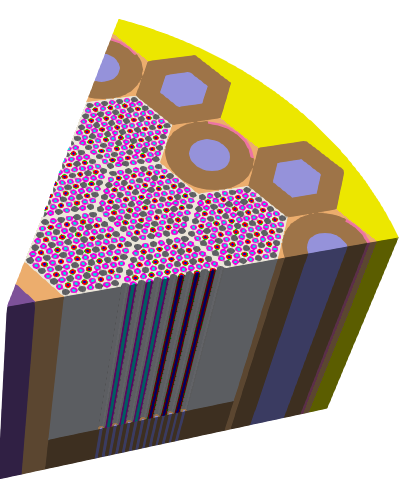
\includegraphics[scale=0.65]{images/VTB_fullcore_3D_slice_sextant.png}  % Modifica scale o usa width se serve
\caption{3D sketch of the HPMR core, considering only one sextant of the geometry.}
\label{fig:VTB_fullcore_3D_slice_sextant}
\end{figure}


\section{Methodology} \label{section:Methodology}

This section begins with a description of the fission matrix method, followed by the definition of the FM database. The interpolation procedure is then presented.
Since higher errors are observed when a large temperature difference between the core and the reflector occurs, a Reflector Correction Ratio (RCR) is introduced and described. Furthermore, a correlation between the total power and the system’s temperature distribution is established and subsequently employed in the criticality search algorithm.

\subsection{The Fission Matrix method} \label{subsection:Fission matrix definition}
In this work, the fission matrix coefficients are generated using the Serpent 2 Monte Carlo code \cite{LEPPANEN2025}.
To define the fission matrix, the user is required to discretize the Serpent model into $N$ spatial cells, each used to tally the average number of neutrons produced in the $i$-th cell as a result of a fission event initiated by a neutron born in the $j$-th cell. This set of interactions is stored in a $N \times N$ matrix $\textbf{A}$, known as the \textit{fission matrix}. In multiplying systems, the dominant eigenvector $F_0(\vec{r})$ (denoted as $F$ from now on for simplicity) of $\textbf{A}$ represents the steady-state fission source distribution. Similarly, its associated eigenvalue corresponds to the effective multiplication factor, $k_{eff}$ \cite{Carney2014}. The eigenproblem can then be formulated as follows,

\begin{equation}
F_i = \frac{1}{k_{eff}}\sum_j^N a_{ij}F_j,
\label{eq:fission_matrix_eigenproblem}
\end{equation}
where $a_{ij}$ is the coefficient of $\textbf{A}$ in the $i$-th row and $j$-th column. Once the FM is assembled, the fission source and the associated eigenvalue can be easily computed numerically with an eigenvalue solver; in this study the eigenproblem solver included in the python package scipy is adopted \cite{2020SciPy-NMeth}.
Serpent 2 tallies the fission matrix on a Cartesian mesh. This is convenient for a square-lattice system, where the mesh cells can be made to overlap the actual position of the fissile elements, whether at pin or at assembly level, but it is not suited to the hexagonal lattice of the HPMR. 
To overcome this limitation, the Serpent 2 capability to tally the fission matrix in each fissile material was exploited. The core has 30 fuel assemblies and 3 axial regions have been defined to improve the axial results resolution for this study; hence, the mesh consists of 90 cells, yielding a fission matrix with $90 \times 90 = 8100$ elements. \rthree{\linelabel{rl:r3_3d}It is important to stress that the resulting discretization is fully three-dimensional: the indices $i$ and $j$ do not refer to a radial mesh, but to three-dimensional cells obtained by combining the radial position of the assembly with its axial region. Every quantity defined on the fission matrix in the following, including the correction introduced in \cref{subsection:Core reflector treatment}, therefore connects two three-dimensional regions, and the radial and axial effects are treated simultaneously rather than being separated into distinct factors.}


\subsection{FM Database Definition} \label{subsection:Database definition}
The FM method requires a certain upfront computational burden to generate the Fission Matrix Database (FMDB), with the advantage of using the pre-computed data to generate an interpolated FM that represents any arbitrary core configuration. The computational resources required clearly depend both on the number of parameters relevant for the system's analysis and on the level of accuracy targeted.
In this work, two key parameters are considered: the system temperature and the angular position of the control drums.

It is important to specify that each temperature value in the database (corresponding to one database entry) represents a uniform temperature applied to the entire reactor system. That is, no spatial temperature gradients are considered when generating the database, assuming that fuel, moderator, and structural components are at the same temperature. Similarly, the CD position is represented by a single rotation angle for all the control drums, preserving a symmetric control strategy.

One of the challenges of defining the FMDB is that the minimum amount of data (and, hence, database entries) needed to produce sufficiently accurate results is not known \textit{a priori}. Therefore, an analysis of the optimal number of database entries for the analyzed system is presented in the Results section.   

\subsection{FM Interpolation}
Since the FMDB depends on two variables, a bi-variate interpolation scheme is required. As a starting point, it was natural to select a simple bi-variate linear interpolation. More advanced interpolation schemes, beyond the scope of this work, will be considered in future studies to optimize the amount of data needed in the FMDB.

The bi-variate linear interpolation used to obtain the element $\tilde{a}_{ij}$ of the interpolated fission matrix $\tilde{\mathbf{A}}$ is defined as

\begin{align}
\tilde{a}_{ij}(\tilde{T}_{f,i}, \tilde{\theta}) =&\; a_{ij}^{(d_T, d_{\theta})}
\left( \frac{T_{f,i}^{(d_T+1)} - \tilde{T}_{f,i}}{T_{f,i}^{(d_T+1)} - T_{f,i}^{(d_T)}} \right)
\left( \frac{\theta^{(d_{\theta}+1)} - \tilde{\theta}}{\theta^{(d_{\theta}+1)} - \theta^{(d_{\theta})}} \right) \notag \\
&+ a_{ij}^{(d_T+1, d_{\theta})}
\left( \frac{\tilde{T}_{f,i} - T_{f,i}^{(d_T)}}{T_{f,i}^{(d_T+1)} - T_{f,i}^{(d_T)}} \right)
\left( \frac{\theta^{(d_{\theta}+1)} - \tilde{\theta}}{\theta^{(d_{\theta}+1)} - \theta^{(d_{\theta})}} \right) \notag \\
&+ a_{ij}^{(d_T, d_{\theta}+1)}
\left( \frac{T_{f,i}^{(d_T+1)} - \tilde{T}_{f,i}}{T_{f,i}^{(d_T+1)} - T_{f,i}^{(d_T)}} \right)
\left( \frac{\tilde{\theta} - \theta^{(d_{\theta})}}{\theta^{(d_{\theta}+1)} - \theta^{(d_{\theta})}} \right) \notag \\
&+ a_{ij}^{(d_T+1, d_{\theta}+1)}
\left( \frac{\tilde{T}_{f,i} - T_{f,i}^{(d_T)}}{T_{f,i}^{(d_T+1)} - T_{f,i}^{(d_T)}} \right)
\left( \frac{\tilde{\theta} - \theta^{(d_{\theta})}}{\theta^{(d_{\theta}+1)} - \theta^{(d_{\theta})}} \right),
\end{align}

where the individual terms are identified as follows:
\begin{itemize}
  \item $\tilde{a}_{ij}$: interpolated element of the fission matrix $\tilde{\mathbf{A}}$,
  \item $d_T$, $d_{\theta}$: indices such that $\tilde{T}_f \in [T_f^{(d_T)}, T_f^{(d_T+1)}]$ and $\tilde{\theta} \in [\theta^{(d_{\theta})}, \theta^{(d_{\theta}+1)}]$  ,
  \item $a_{ij}^{(d_T, d_{\theta})}$: FM element entry at grid point $(T_f^{(d_T)}, \theta^{(d_{\theta})})$ of the FMDB,
  \item $\tilde{T}_{f,i}$: fuel temperature of target cell "$i$" for interpolation,
  \item $\tilde{\theta}$: target CD angle,
  \item $T_f^{(d_T)}$, $T_f^{(d_T+1)}$: adjacent temperature grid points in the FMDB,
  \item $\theta^{(d_{\theta})}$, $\theta^{(d_{\theta}+1)}$: adjacent angle grid points in the FMDB.
\end{itemize}

Notice that from now on, the tilde symbol (\textasciitilde) is adopted for referring to interpolated variables.   

\subsection{Core Reflector Treatment: Definition of the Reflector Correction Ratio} \label{subsection:Core reflector treatment}
In nuclear reactors, neutron reflectors are employed to reduce neutron leakage by scattering escaping neutrons back into the core, thereby enhancing the overall neutron economy. This allows for more efficient fuel utilization and contributes to maintaining criticality with less fissile material. In microreactors, reflectors play an even more important role due to the compactness of the core and the limited amount of fissile material, strongly affecting the neutron flux shape.

Due to the definition of the fission matrix cells in this work, temperature can only be imposed on the fuel assemblies during interpolation. Moreover, the database used in this study assumes a uniform temperature distribution across the entire system. As a result, when analyzing more realistic cases that include a temperature gradient between the fuel and the reflector, the method may yield less accurate results. To address this limitation, a Reflector Correction Ratio (RCR) is defined. This approach is similar to the one adopted in \cite{Rau2020} but focuses on the definition and application of the correction to the temperature difference between core and reflector, which plays a crucial role in HPMRs. The reference approach consists in multiplying each element of $\tilde{\textbf{A}}$, by the corresponding elements of $\textbf{R}$, which contains the correction ratios,  $r_{i,j}$,  of each element of the fission matrix, such that: 

\begin{equation}
F_i = \frac{1}{\tilde{k}_{eff}}\sum_j \tilde{a}_{i,j}^{*}F_j = \frac{1}{\tilde{k}_{eff}}\sum_j r_{i,j}\tilde{a}_{i,j}F_j.
\label{eq:fission_source_with_correction_calculation}
\end{equation}

The coefficients, $r_{i,j}$ of $\textbf{R}$ are defined as follows:

\begin{equation}
\rtwocolor r_{i,j}(\Delta T_i, \Delta T_j, \theta) = \frac{1}{2}\,\frac{\Delta T_i + \Delta T_j}{T_{max,DB} - T_{min,DB}} \cdot \left( \frac{ a_{i,j}^{\Delta T}}{\tilde{a}_{i,j}(T_{f,i}, \theta)} - 1 \right) + 1
\label{eq:correction_ratio_1}
\end{equation}

with each of the terms defined as follows:

\begin{itemize}
    \item \rtwo{$\Delta T_k = T_{f,k} - T_{r,k}$: local temperature difference of the fissile cell '$k$', where $T_{r,k}$ is the temperature of the closest non-fissile cell.}
    \item $ \theta $: CD rotation angle.
    \item $T_{max,DB}$: maximum temperature used to generate the database.
    \item $T_{min,DB}$: minimum temperature used to generate the database
    \item $a_{i,j}^{\Delta T}$: fission matrix generated with $T_{f}=1000$K and $T_{r}=300$K.
\end{itemize}

\linelabel{rl:derivation}\rtwo{The structure of \cref{eq:correction_ratio_1} follows from the role that the reflector plays in the neutron balance of the system. The reflector enters this balance because the neutrons born in a peripheral cell leak out of the active region, interact with the reflector, and a fraction of them is scattered back into the core, where they induce further fissions. This process involves both cells of a general coefficient $a_{i,j}$, the one in which the neutrons are born and the one in which the fissions are induced, and the ratio between the two fission matrices retains the dependence on both indices.}

\linelabel{rl:assumptions}\rtwo{Two assumptions are introduced in \cref{eq:correction_ratio_1}. The first one is that the departure of each coefficient from its uniform-temperature value scales linearly with the local temperature difference between fuel and reflector, so that the whole correction can be expressed through the single reference case $a_{i,j}^{\Delta T}$ instead of requiring a dedicated database entry for each temperature gradient. The second one concerns the localization of the weight. Since a coefficient describes a transfer between two cells, each surrounded by its own thermal environment, the local temperature difference entering the weight is taken as the average of the differences of the two cells. For each cell, $T_{r,k}$ is the temperature of the closest non-fissile region. The interpolated coefficient appearing at the denominator is instead evaluated at the temperature of the receiving cell. Formulations in which the weight depends on a single index have also been verified. They coincide with the present one whenever the local temperature difference is spatially uniform, and differ only in the cases with a non-uniform distribution; the selected weight formulation yields the smallest deviations on the multiplication factor. This approach originates from the correction ratio introduced in \cite{He2019}, where a single-index form is used; there, however, the correction factor is obtained as a ratio of fission rates tallied at a given position under an imposed uniform source, and is therefore a single-index quantity by construction, whereas the ratio adopted here is the ratio of two complete fission matrices.}

\linelabel{rl:limits}\rtwo{The behaviour of \cref{eq:correction_ratio_1} in the limiting cases follows directly from its definition. When the fuel and the reflector are at the same temperature in both cells, $T_{f,i} = T_{r,i}$ and $T_{f,j} = T_{r,j}$, the weight vanishes and $r_{i,j} = 1$, so that the interpolated matrix is left unchanged. This is the expected result, since in this condition the assumption of a uniform temperature distribution used to generate the database is exactly satisfied. When the temperature difference in both cells corresponds to the one adopted for the correction reference case, that is $T_{f,i} = T_{f,j} = T_{max,DB} = 1000$ K and $T_{r,i} = T_{r,j} = T_{min,DB} = 300$ K, the weight is equal to unity and the corrected coefficient reduces to}

\begin{equation}
\rtwocolor \tilde{a}_{i,j}^{*} = r_{i,j} \, \tilde{a}_{i,j} = a_{i,j}^{\Delta T},
\label{eq:correction_limiting_case}
\end{equation}

\rtwo{recovering exactly the fission matrix computed with the reference temperature gradient. Between these two limits the correction varies linearly with the mean of the two local temperature differences.}

Based on the proposed formulation from \cref{eq:correction_ratio_1}, an additional Monte Carlo calculation is required to obtain $a_{i,j}^{\Delta T}$ to calculate the correction ratio. Although negligible, this additional case has to be considered as an extra computational effort to the FMDB generation process.  
The RCR defined in \cref{eq:correction_ratio_1} only accounts for temperature effects. HPMRs typically adopt a control mechanism that uses control drums located outside of the core, within the reflector region. This design choice significantly influences the neutron flux distribution, particularly at the interface between the reflector and the outermost ring of fuel assemblies. When the control drums are rotated towards the core to increase the neutron absorption in the reflector region, a pronounced perturbation in the local neutron spectrum and leakage occurs in this boundary region. Thus, each time a CD is rotated, the relation between the reflector and the core changes, requiring a new $a_{i,j}^{\Delta T}$ to describe the new configuration of the control drums combined with the temperature difference between the active region and the reflector. 
Since this effect is not negligible, the RCR introduced in \cref{eq:correction_ratio_1} is redefined to account for the control drum insertion as follows:    

\begin{equation}
\rtwocolor r_{i,j}(\Delta T_i, \Delta T_j, \theta) = \frac{1}{2}\,\frac{\Delta T_i + \Delta T_j}{T_{max,DB} - T_{min,DB}} \cdot \left( \frac{ \tilde{a}_{i,j}^{\Delta T}(\theta)}{\tilde{a}_{i,j}(T_{f,i}, \theta)} - 1 \right) + 1
\label{eq:correction_ratio_2}
\end{equation}

With respect to the original formulation in \Cref{eq:correction_ratio_1}, it is important to note that the coefficient $\tilde{a}_{i,j}^{\Delta T}$ is now a function of the parameter $\theta$. This dependency arises from the combined effect of the thermal gradients and control drum absorber configuration within the reflector.

As a direct consequence, the numerator of the RCR must also be interpolated across different values of $\theta$. This modification introduces a significant refinement in the correction mechanism, as it adapts more effectively to the angular variation of the system's response. \linelabel{rl:eq5note}\rtwo{The limiting cases discussed for \cref{eq:correction_ratio_1} are preserved, since at a given drum position the reference coefficient $\tilde{a}_{i,j}^{\Delta T}(\theta)$ plays the same role as $a_{i,j}^{\Delta T}$ in the first formulation.}

As a result, the total number of simulations required to construct the database and compute the RCR using the second formulation is:
\begin{equation}
    N_T N_{\theta} + N_{\theta},
\end{equation}

where $N_T$ and $N_{\theta}$ are the number of fuel temperature and control drum angle values of the database.

%Equation \cref{eq:correction_ratio_2} is more expansive from the computational time point of view then the first formulation, however it is important to stress the fact that for control rods-based reactor designs, \cref{eq:correction_ratio_1} would be enough to improve results accuracy, since the peripheral region outside the core does not change during the operations of the reactor. The control rods are inserted inside the core to tune the reactivity of the system, which for sure causes strong neutron flux changes, and thus the FM's values, however these effects would be already accounted when different insertion steps are simulated to build the the FMDB.      


\subsection{Power and fuel temperature correlation}
\label{subsec:Power and fuel temperature correlation}
To estimate an average fuel temperature corresponding to a given power level without performing a full thermal-hydraulic simulation for each case, which is out of the scope of this work, an arbitrary correlation is defined. This approach is used to generate a mockup temperature distribution for the HPMR model as a direct function of the reactor power. The distribution is then used for the interpolation of the fission matrix coefficients. The correlation effectively introduces a simple dependency between the power level and the fuel temperature used in the FM model, eliminating the need for a full thermal hydraulic calculation.

\rthree{\linelabel{rl:r3_thermal}It is worth clarifying that no thermal calculation is performed in this work, and that neither a conduction model nor a heat pipe model is therefore described. The temperature distributions adopted in all the test cases are prescribed inputs, defined either analytically, as in the cases with imposed gradients, or through the correlation introduced in this section. This choice does not affect the assessment of the method, because the reference Serpent 2 calculations are performed with exactly the same prescribed temperature distributions. The deviations reported in \cref{section:Results and discussion} therefore measure the accuracy of the fission matrix interpolation and of the reflector correction, and not the accuracy of a thermal model. The coupling of the proposed method with a dedicated thermal model, and in particular with a heat pipe model, is left to future developments.}

Assuming that the average fuel temperature scales linearly with power and that the temperature distribution itself is proportional to the fission source ($T_{f,i} \propto F_{i} $), the following correlation is defined:


\begin{align}
 &T_{f,i} =  \frac{P}{P_N} \xi_i  + T_{\min,DB},
\label{eq:correction_power_temperature} \\ &
\xi_i= \left[ \frac{\tilde{F}_i - \min(\tilde{F})}{\max(\tilde{F}) - \min(\tilde{F})} \cdot \Delta T_{\text{range}} + (T_{f,\min} - T_{\min,DB}) \right],
\notag \\ &
 \text{with} \quad P \in [0,P_{\text{max}}]. \notag
\end{align}


where: 

\begin{itemize}
    \item $P$: is the reactor power and is an independent (input) variable.
    \item $P_N$: is the nominal power of the reactor (2 MW). 
    \item $T_{f,i}$: temperature of the fissile cell '$i$'. 
    \item $\Delta T_{range} $: is the maximum temperature difference within the core at nominal power. 
    \item $T_{f,min}$: is the minimum temperature encountered inside the core at nominal power. Both parameters have to be provided as inputs.  
    \item $T_{min,DB}$: minimum temperature used to generate the database.   
\end{itemize}

This formulation is subject to a specific range of validity, as the power level must not exceed an upper bound, denoted as \( P_{\text{max}} \). This constraint ensures that the resulting fuel temperature does not exceed the maximum temperature present in the database, which is limited to \( T_{\text{max,DB}} = 1000\,\text{K} \). The maximum allowable power is defined as follows:

\begin{equation}
P_{\text{max}} = \frac{(T_{\text{max,DB}} - T_{\text{min,DB}})\cdot P_N}{\Delta T_{\text{range}} + (T_{\text{f,min}} - T_{\text{min,DB}})}
\label{eq:maximum_power_formulation}
\end{equation}

% Thus, the maximum allowable input power depends on two parameters: $\Delta T_{\text{range}}$ and $T_{\text{f,min}}$. In \Cref{fig:parametric_limits_Pmax}, the parametric variation of the system’s upper power limit is shown. Once the parameters are chosen, all the points above the resulting curves would make the temperature distribution exceed the maximum temperature considered when generating the database (1000 K). Conversely, all points below the curve ensure that the temperature in every cell remains within the valid range of the database. Note that, if values above $P_{\text{max}}$ are needed or expected, additional entries in the database at higher uniform temperatures can be introduced.

% \begin{figure}[h!]
% \centering
% 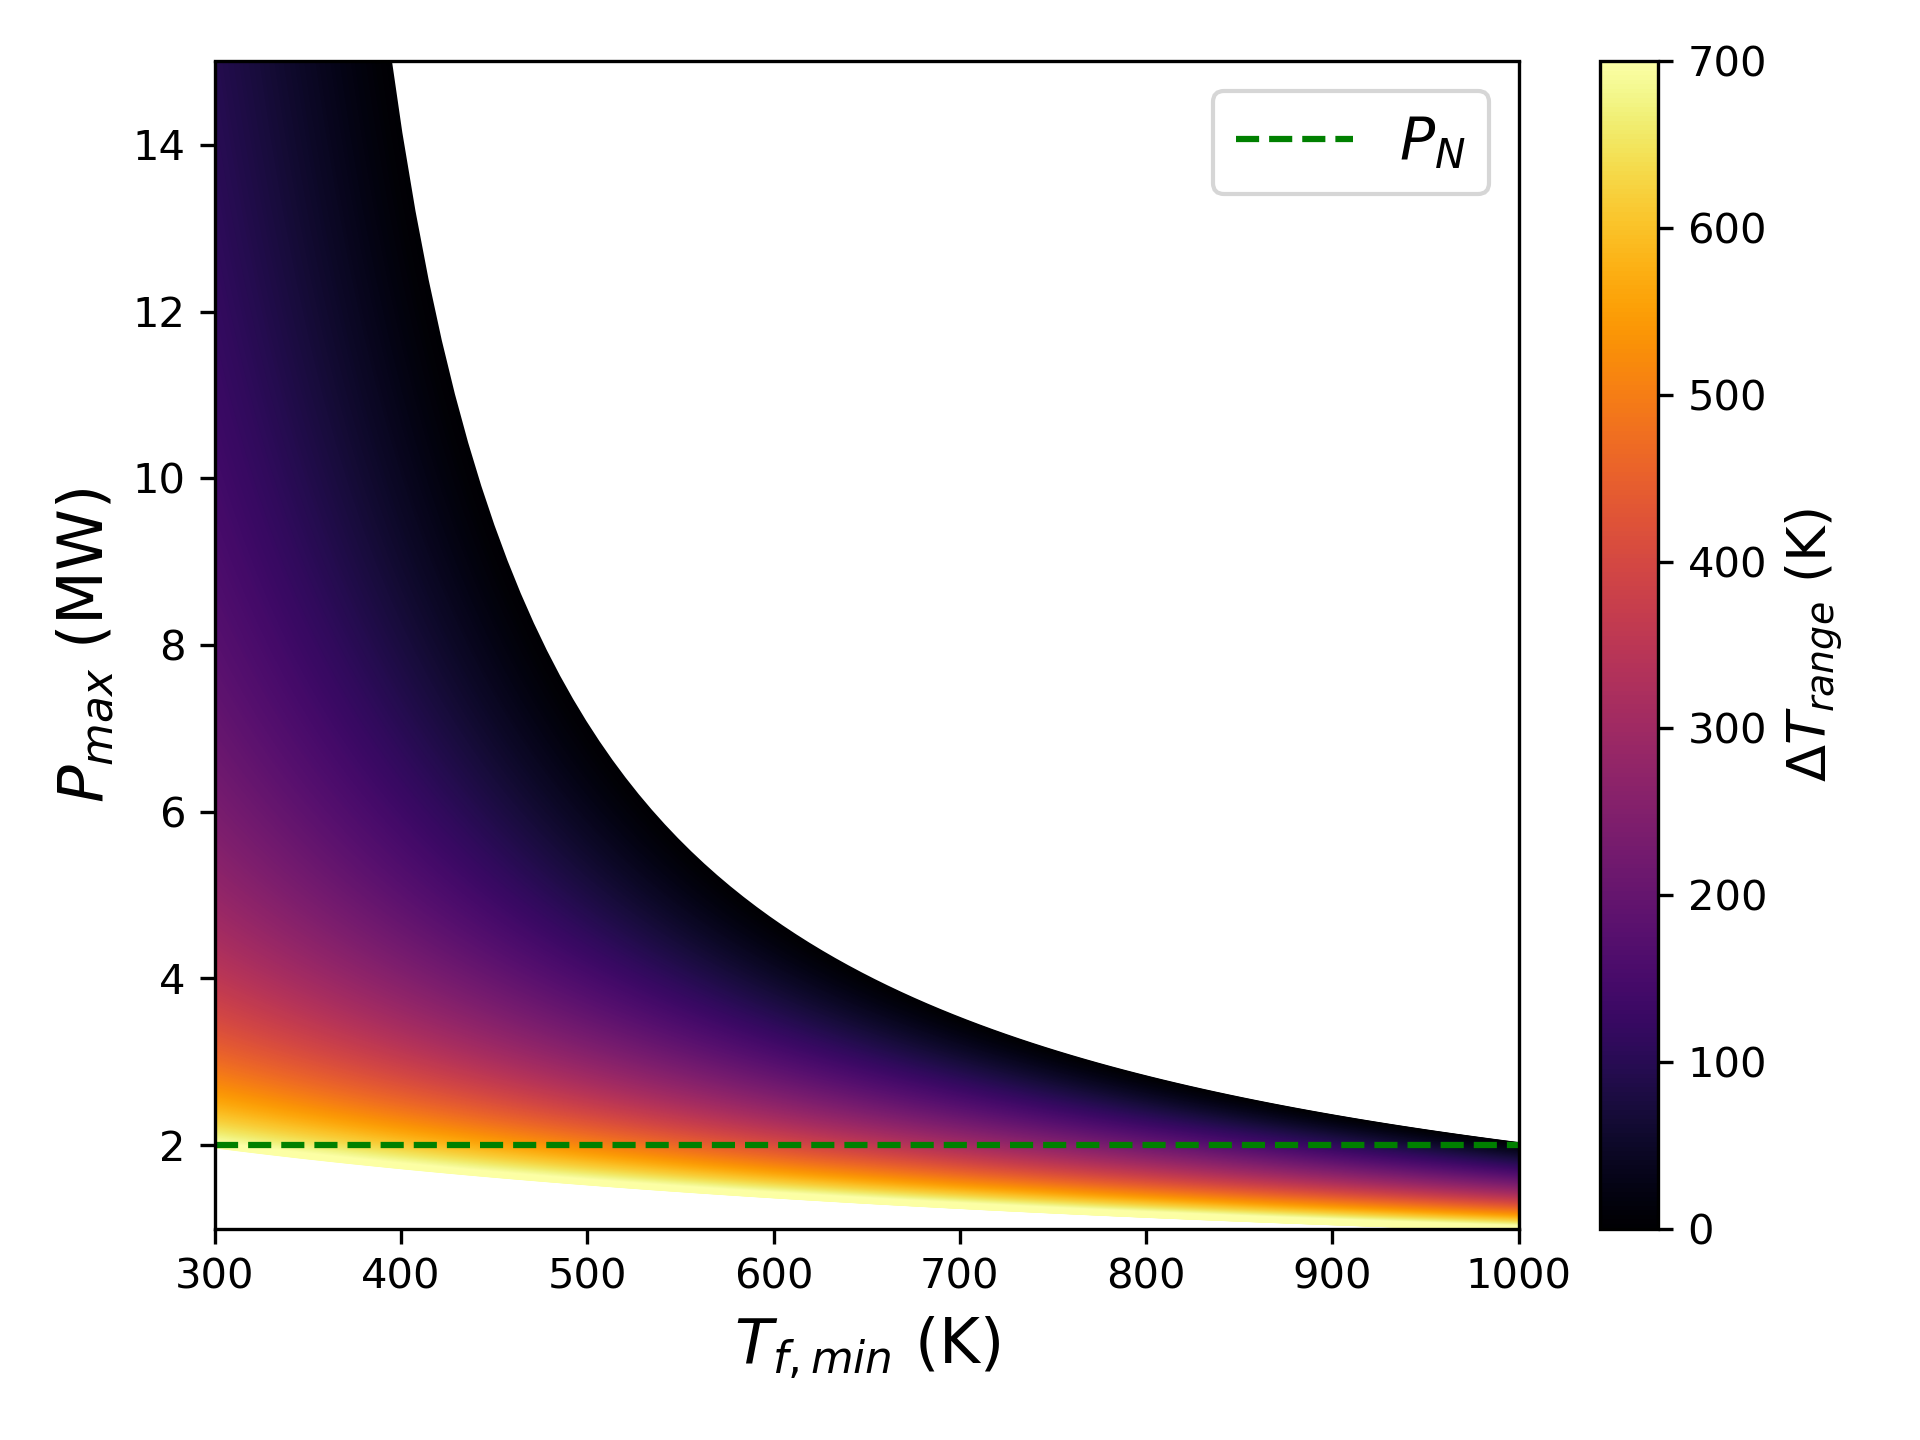
\includegraphics[scale=0.5]{images/parametric_limits_Pmax.png}  % Modifica scale o usa width se serve
% \caption{Parametric $P_{\text{max}}$ domain visualization.}
% \label{fig:parametric_limits_Pmax}
% \end{figure}


\subsection{Criticality search algorithm}
\label{subsec:criticality_search_method}
Thanks to the correlation previously defined between power and fuel temperature, it is now possible to automate both the computation of the temperature distribution within the fuel and the criticality search involving the control drum positioning.

The criticality search algorithm aims at determining a configuration of the system in which the reactor reaches a critical state (i.e., $k_{eff} = 1$), while accounting for the thermal feedback on the neutron flux and the CD positions. The procedure includes two nested convergence loops: one for the temperature distribution and one for the reactor's criticality itself. The algorithm steps, corresponding to the flowchart in \Cref{fig:crit_search_unified_loop}, are described below:

% \begin{enumerate}
%     \item \textbf{Initialization:} \\
%     The algorithm begins by setting the CD angle $\theta_{CD} = 0$, an initial guess for the fission source distribution $F_{\text{guess}}$, the minimum fuel temperature $T_{f,min}$, the maximum temperature difference observed inside the system, $\Delta T_{\text{range}}$, and the total power $P$.

%     \item \textbf{Initial temperature calculation:} \\
%     Based on the initial guess, the corresponding fuel temperature distribution $T_f$ is computed, using \cref{eq:correction_power_temperature}.

%     \item \textbf{Fission source distribution calculation:} \\
%     With the current temperature field, a new fission source distribution $\tilde{F}$ is computed using the FM interpolation.

%     \item \textbf{Updated Temperature Calculation:} \\
%     A new temperature profile is calculated using the updated fission source distribution, $\tilde{F}$, considering thermal feedback.

%     \item \textbf{Temperature Convergence Check:} \\
%     The algorithm checks whether the new temperature profile differs from the previous by less than a defined threshold, $\epsilon$. In this study $\epsilon$ is set to 0.5\%. If this convergence criterion is not satisfied:
%     \begin{itemize}
%         \item The temperature profile is updated.
%         \item The algorithm returns to step 3 and continues iterating.
%     \end{itemize}
%     If convergence is achieved, the algorithm proceeds to the next step.

%     \item \textbf{Criticality Convergence Check:} \\
%     The previous $\tilde{k}_{eff}^{old}$ is updated with the current $\tilde{k}_{eff}^{new}$. The convergence condition $|\tilde{k}_{eff}^{new} - 1| < \delta$ is then checked:
%     \begin{itemize}
%         \item If not satisfied, the CD angle is adjusted and the algorithm returns to step 3.
%         \item If satisfied, criticality is achieved, and the algorithm proceeds to the final step.
%     \end{itemize}
%     In this study $\delta$ is set to 1 pcm. 

%     \item \textbf{Finalization:} \\
%     Once both the temperature and criticality convergence conditions are met, the final configuration is saved, including the critical temperature distribution, the critical power profile, and the critical control drum angle.
% \end{enumerate}


\begin{enumerate}
    \item \textbf{Initialization:} \\
    The algorithm begins by setting the CD angle $\theta_{CD} = 0$, an initial guess for the fission source distribution $F_{\text{guess}}$, the minimum fuel temperature $T_{f,min}$, the maximum temperature difference observed inside the system $\Delta T_{\text{range}}$, and the total power $P$.

    \item \textbf{NE--TH equilibrium calculation:} \\
    The coupled neutronic–thermal-hydraulic equilibrium is solved iteratively as follows:

    \begin{enumerate}
        \item \textbf{Initial temperature calculation:} \\
        Based on the current fission source estimate, the fuel temperature distribution $T_f$ is computed using \cref{eq:correction_power_temperature}.

        \item \textbf{Fission source distribution calculation:} \\
        Using the updated temperature field, a new fission source distribution $\tilde{F}$ is computed via FM interpolation.

        \item \textbf{Updated temperature calculation:} \\
        A new temperature profile is computed using the updated fission source distribution $\tilde{F}$, including thermal feedback effects.

        \item \textbf{Temperature convergence check:} \\
        The algorithm checks whether the new temperature profile differs from the previous one by less than a defined threshold $\epsilon$ (here $\epsilon = 0.5\%$). If convergence is not reached:
        \begin{itemize}
            \item update the temperature profile;
            \item return to step 2.2.
        \end{itemize}
    \end{enumerate}

    \item \textbf{Criticality convergence check:} \\
    The previous $\tilde{k}_{eff}^{old}$ is updated with the current $\tilde{k}_{eff}^{new}$. The convergence condition
    $|\tilde{k}_{eff}^{new} - 1| < \delta$ is checked, with $\delta = 1$ pcm.
    \begin{itemize}
        \item If not satisfied, the CD angle is adjusted and the algorithm returns to step 2.
        \item If satisfied, criticality is achieved and the algorithm proceeds.
    \end{itemize}

    \item \textbf{Finalization:} \\
    Once both temperature and criticality convergence conditions are met, the final configuration is saved, including the critical temperature distribution, the critical power profile, and the critical control drum angle.
\end{enumerate}


\begin{figure}[h!]
\centering
\scalebox{0.60}{
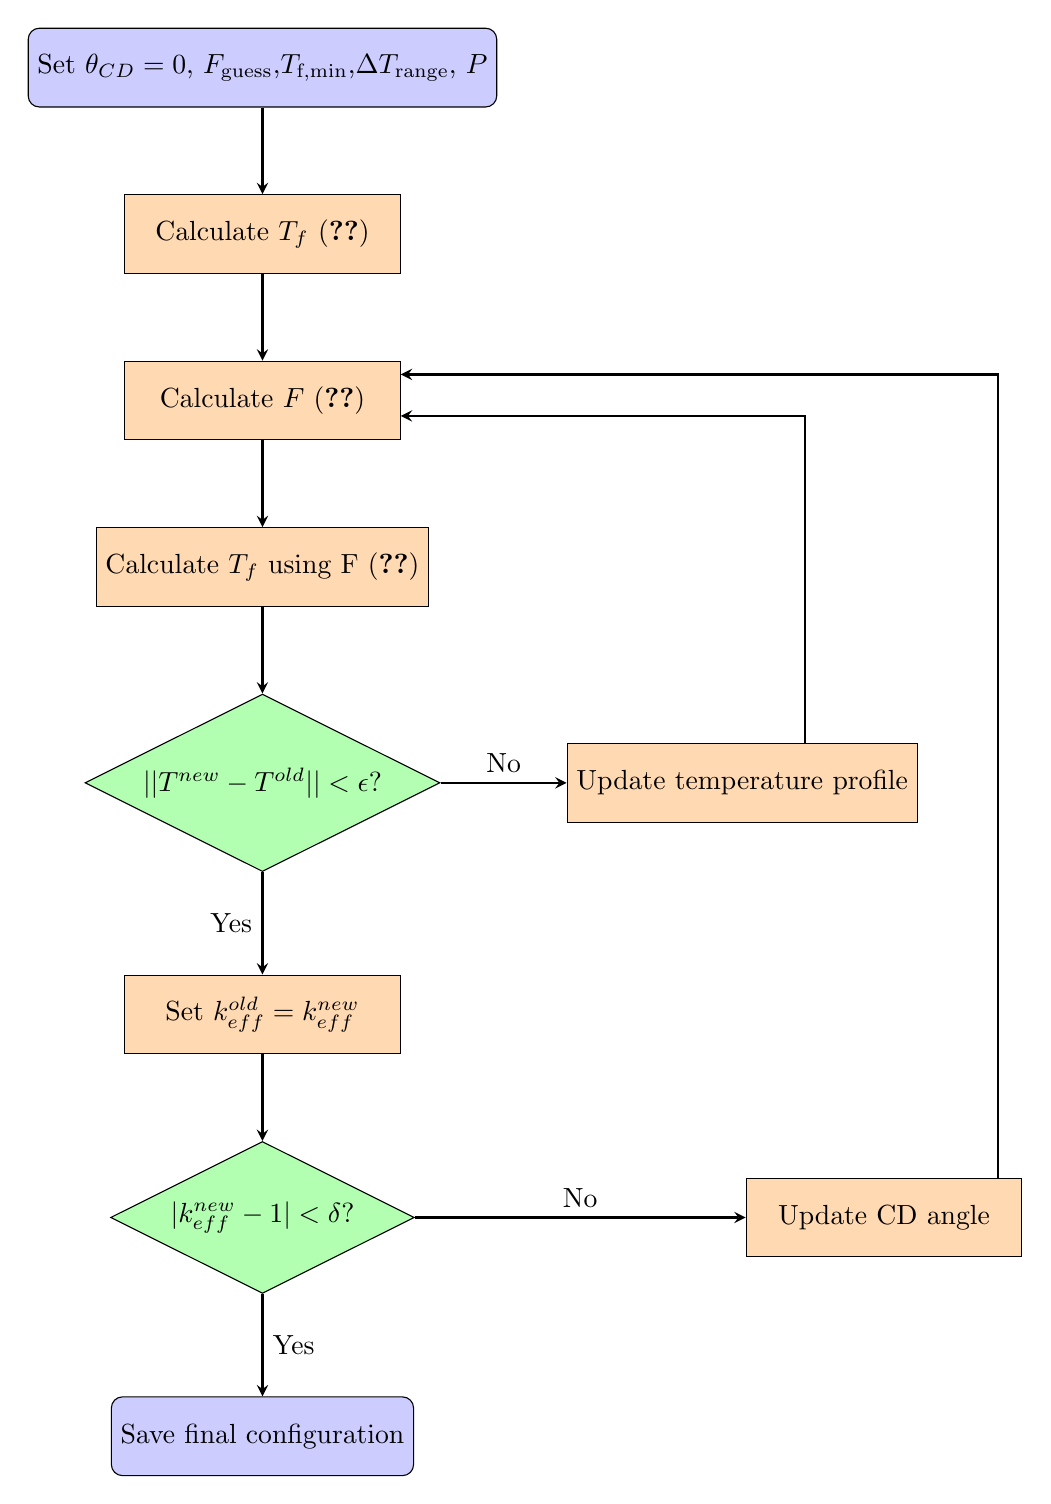
\begin{tikzpicture}[node distance=1.1cm and 1.6cm]

% Nodi principali
\node (start) [startstop] {Set $\theta_{CD} = 0$, $F_{\text{guess}}$,$T_{\text{f,min}}$,$\Delta T_{\text{range}}$, $P$};
\node (calcT1) [process, below=of start] {Calculate $T_f$  (\cref{eq:correction_power_temperature})};

\node (calcF) [process, below=of calcT1] {Calculate $F$ (\cref{eq:fission_source_with_correction_calculation})};

\node (calcT2) [process, below=of calcF] {Calculate $T_f$ using F (\cref{eq:correction_power_temperature})};


\node (tempConv) [decision, below=of calcT2] {$||T^{new} - T^{old}|| < \epsilon$?};
\node (updateT) [process, right=of tempConv, xshift=0.001cm] {Update temperature profile};
\node (returnTempLoop) [coordinate, above=of updateT, yshift=1cm] {};

\node (keffUpdate) [process, below=of tempConv, yshift=-0.2cm] {Set $k_{eff}^{old} = k_{eff}^{new}$};
\node (critConv) [decision, below=of keffUpdate] {$|k_{eff}^{new} - 1| < \delta$?};
\node (updateCD) [process, right=of critConv, xshift=2.6cm] {Update CD angle};
\node (end) [startstop, below=of critConv, yshift=-0.2cm] {Save final configuration};

% Flussi
\draw [arrow] (start) -- (calcT1);
\draw [arrow] (calcT1) -- (calcF);
\draw [arrow] (calcF) -- (calcT2);
\draw [arrow] (calcT2) -- (tempConv);

% Ciclo temperatura
\draw [arrow] (tempConv) -- node[above] {No} (updateT);
\draw [arrow] (updateT.north) ++(0.8,0) |- ([yshift=-20pt]calcF.north east);


% Dopo convergenza temperatura
\draw [arrow] (tempConv) -- node[left] {Yes} (keffUpdate);
\draw [arrow] (keffUpdate) -- (critConv);

% Ciclo esterno CD
\draw [arrow] (critConv) -- node[above] {No} (updateCD);
% \draw [arrow] (updateCD) |- (calcF);
\draw [arrow] (critConv) -- node[right] {Yes} (end);
\draw [arrow] (updateCD.north)  ++(1.45,0) |- ([yshift=-5pt]calcF.north east);

\end{tikzpicture}
}
\caption{Flowchart of the criticality search algorithm with unified loop returning to the fission source calculation.}
\label{fig:crit_search_unified_loop}
\end{figure}

\subsection{Error metrics applied for accuracy assessment}

In the results section, some test cases are used to quantify the accuracy of the calculations by comparing the results obtained using the FM method to a reference Serpent 2 model. Two main parameters are compared: the $k_{eff}$ and the fission neutron source ($\nu\Sigma_f\phi$ or $F$). The error displayed for the eigenvalue in the results section is defined in \Cref{eq:keff_err}. \Cref{eq:fission_source_rel_err} represents the relative error of the fission source generated using the FM. Finally, \Cref{eq:fission_source_RMS_err} is used to evaluate the Root Mean Square Error of different parameters ($x$), including the fission source relative error (RMSE-$\tilde{F}$). 

To quickly and easily double check the consistency of the fission source results, each Serpent 2 reference case was run three separate times, using different random seeds for each run. For every simulation, the RMSE-$\tilde{F}$ is evaluated to assess how the uncertainty estimation varies depending on the random seed.

The comparison among the three sets of results revealed that the differences are negligible, and all outcomes are fully consistent with one another. This indicates that the stochastic variability introduced by the random seed has little to no impact on the reliability of the fission source estimation, and confirms the robustness of the results.    

\begin{equation}
    \Delta k_{eff} = \left( \tilde{k}_{eff} - k^{MC}_{eff} \right)\cdot 10^{5} \text{ (pcm)}
\label{eq:keff_err}
\end{equation}


\begin{equation}
    e = \frac{\tilde{F}_i-F_i^{MC}}{F_i^{MC}} \cdot 100 \text{ (\%)}
\label{eq:fission_source_rel_err}
\end{equation}


\begin{equation}
    \text{RMSE-X}  = \sqrt{\frac{1}{N} \sum_i^N \left( \frac{\tilde{x}_i-x_{i}^{MC}}{x^{MC}_{i}} \right)^2 }\cdot 100 \text{ (\%)}
\label{eq:fission_source_RMS_err}
\end{equation}


\begingroup\rtwocolor
\subsection{Statistical uncertainty of the interpolated matrix} \label{subsec:Uncertainty}
Comparing the interpolated results with the reference ones is only meaningful if the statistical noise affecting both is quantified, since a residual discrepancy that falls within that noise cannot be interpreted as a modelling bias. Two independent contributions have to be accounted for.

The first one is the statistical uncertainty of the reference calculation, which Serpent 2 reports directly for the multiplication factor and, through the fission source detector, for each cell.

The second one is less immediate. The interpolated matrix is not the outcome of a Monte Carlo simulation of its own: it is a new object, assembled from database matrices that carry finite statistics, and it therefore has no replicas from which an uncertainty could be read off. Its contribution is estimated here by resampling the database. Each database coefficient is treated as a Gaussian variable, centred on its tallied value with standard deviation equal to its tallied uncertainty; a complete realization of the database is drawn, the interpolation and the RCR are both rebuilt from that same realization, and the eigenvalue problem is solved. Five hundred realizations are used.

The two contributions are independent, coming from separate Monte Carlo simulations, and are combined in quadrature, so that each cell carries a total uncertainty $\sigma_{tot,i} = \sqrt{\sigma_{ref,i}^{2} + \sigma_{DB,i}^{2}}$, and the same combination applies to the multiplication factor. Because the fission source is normalized to its sum, the relative uncertainty of each normalized value coincides with that of the corresponding tally, so the relative quantities can be combined directly.

Coefficients are resampled independently of one another, following the uncorrelated variant of the resampling method proposed in \cite{Walters_uncertainty}. Coefficients tallied within the same simulation are in fact correlated, and neglecting this is known to inflate the propagated variance when those correlations are negative; the estimate reported here is therefore a conservative upper bound on the contribution of the database. It is worth stressing that this conservatism acts in the opposite direction when the estimate is used as a significance threshold, since a larger uncertainty makes a residual discrepancy easier to declare compatible with the statistical noise.

\endgroup

\section{Results and discussion} \label{section:Results and discussion}

\subsection{Database selection}

To ensure the accuracy of the FM results while minimizing computational resources, we progressively increase the number of data points in our database. We start with a smaller dataset and then evaluate its adequacy by reproducing a set of reference test cases. If the RMSE of the $k_{eff}$ (RMSE-$k_{eff}$) for these tests does not fall within the acceptable limit (considering $\sigma_{k_{eff}}$ as a reference), we then increase the number of data points, resulting in a larger database (i.e., more entries). 

The test cases used are the same for all the tested databases and are selected by taking the midpoint between two neighboring points of the most refined one. 
The authors acknowledge the existence of more advanced approaches for adaptive data selection strategies; however, a simplified strategy was intentionally adopted to maintain clarity and ease of implementation.

In this study, three databases are tested as displayed in \cref{fig:databases}. The difference between the three databases lies in the number of points considered for the control drums angle, which ranges from 0° to 180° due to the symmetry of their effect beyond this angle. The red crosses indicate the points used for the testing cases. 
In total, eight fuel temperature and seventeen CD angle values are considered in the final database.


\begin{figure}[h!]
\centering
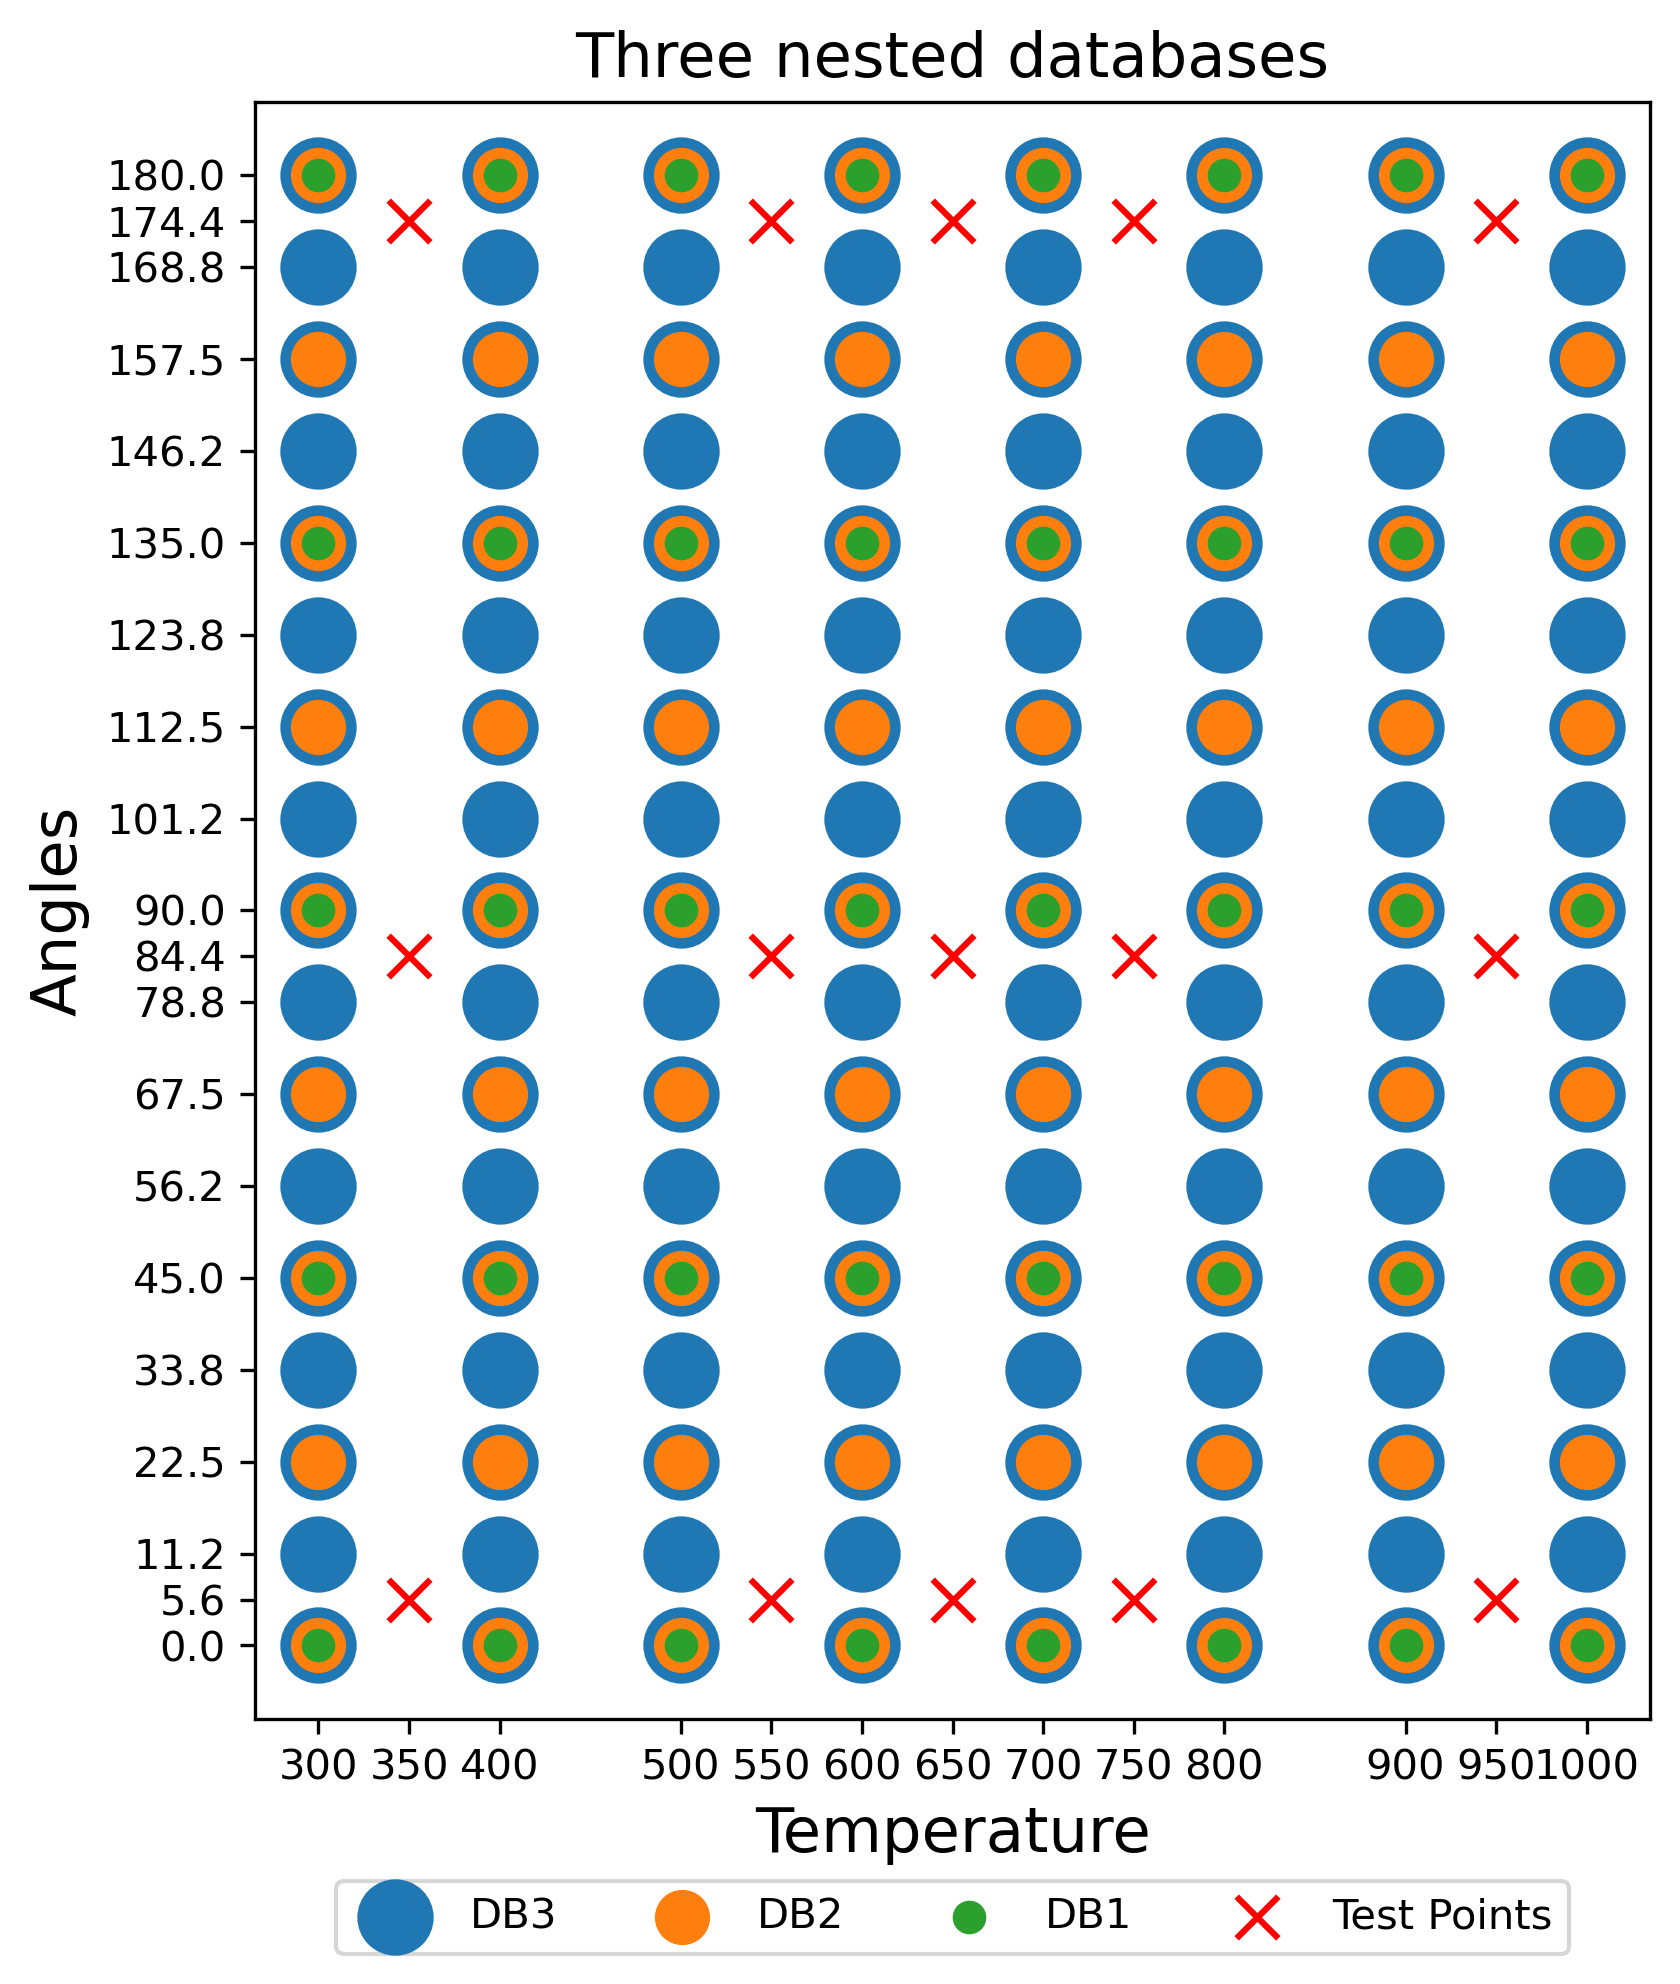
\includegraphics[scale=0.45]{images/nested_databases.png}  % Modifica scale o usa width se serve
\caption{Databases point distribution. The green points are the data of the first and least dense database (Database 1), the orange one is the intermediate one (Database 2), and the blue points are the finest database available (Database 3). The red crosses represent the testing cases.}
\label{fig:databases}
\end{figure}

The reason why only the number of control drum (CD) rotation angles increases between the different databases lies in the stronger and more nonlinear impact of CD rotation on the reactor’s reactivity and, consequently, on the values of the fission matrix, as observed also in \cite{Rau2021Proc}. 

\Cref{fig:linear_interpolation_improvement_changing_database} shows the $\Delta k_{eff}$ between the interpolated fission matrix and the Serpent 2 reference results. The different curves represent the FM database used for the interpolation. As shown, the error of most of the FM simulations reaches a value comparable with the Serpent 2 uncertainty only with Database 3. \Cref{tab:table_delta_k_linear} includes the results of the $\Delta k_{eff}$, along with the maximum $e$, and the RMSE-$\tilde{F}$.

\begin{figure}[h!]
\centering
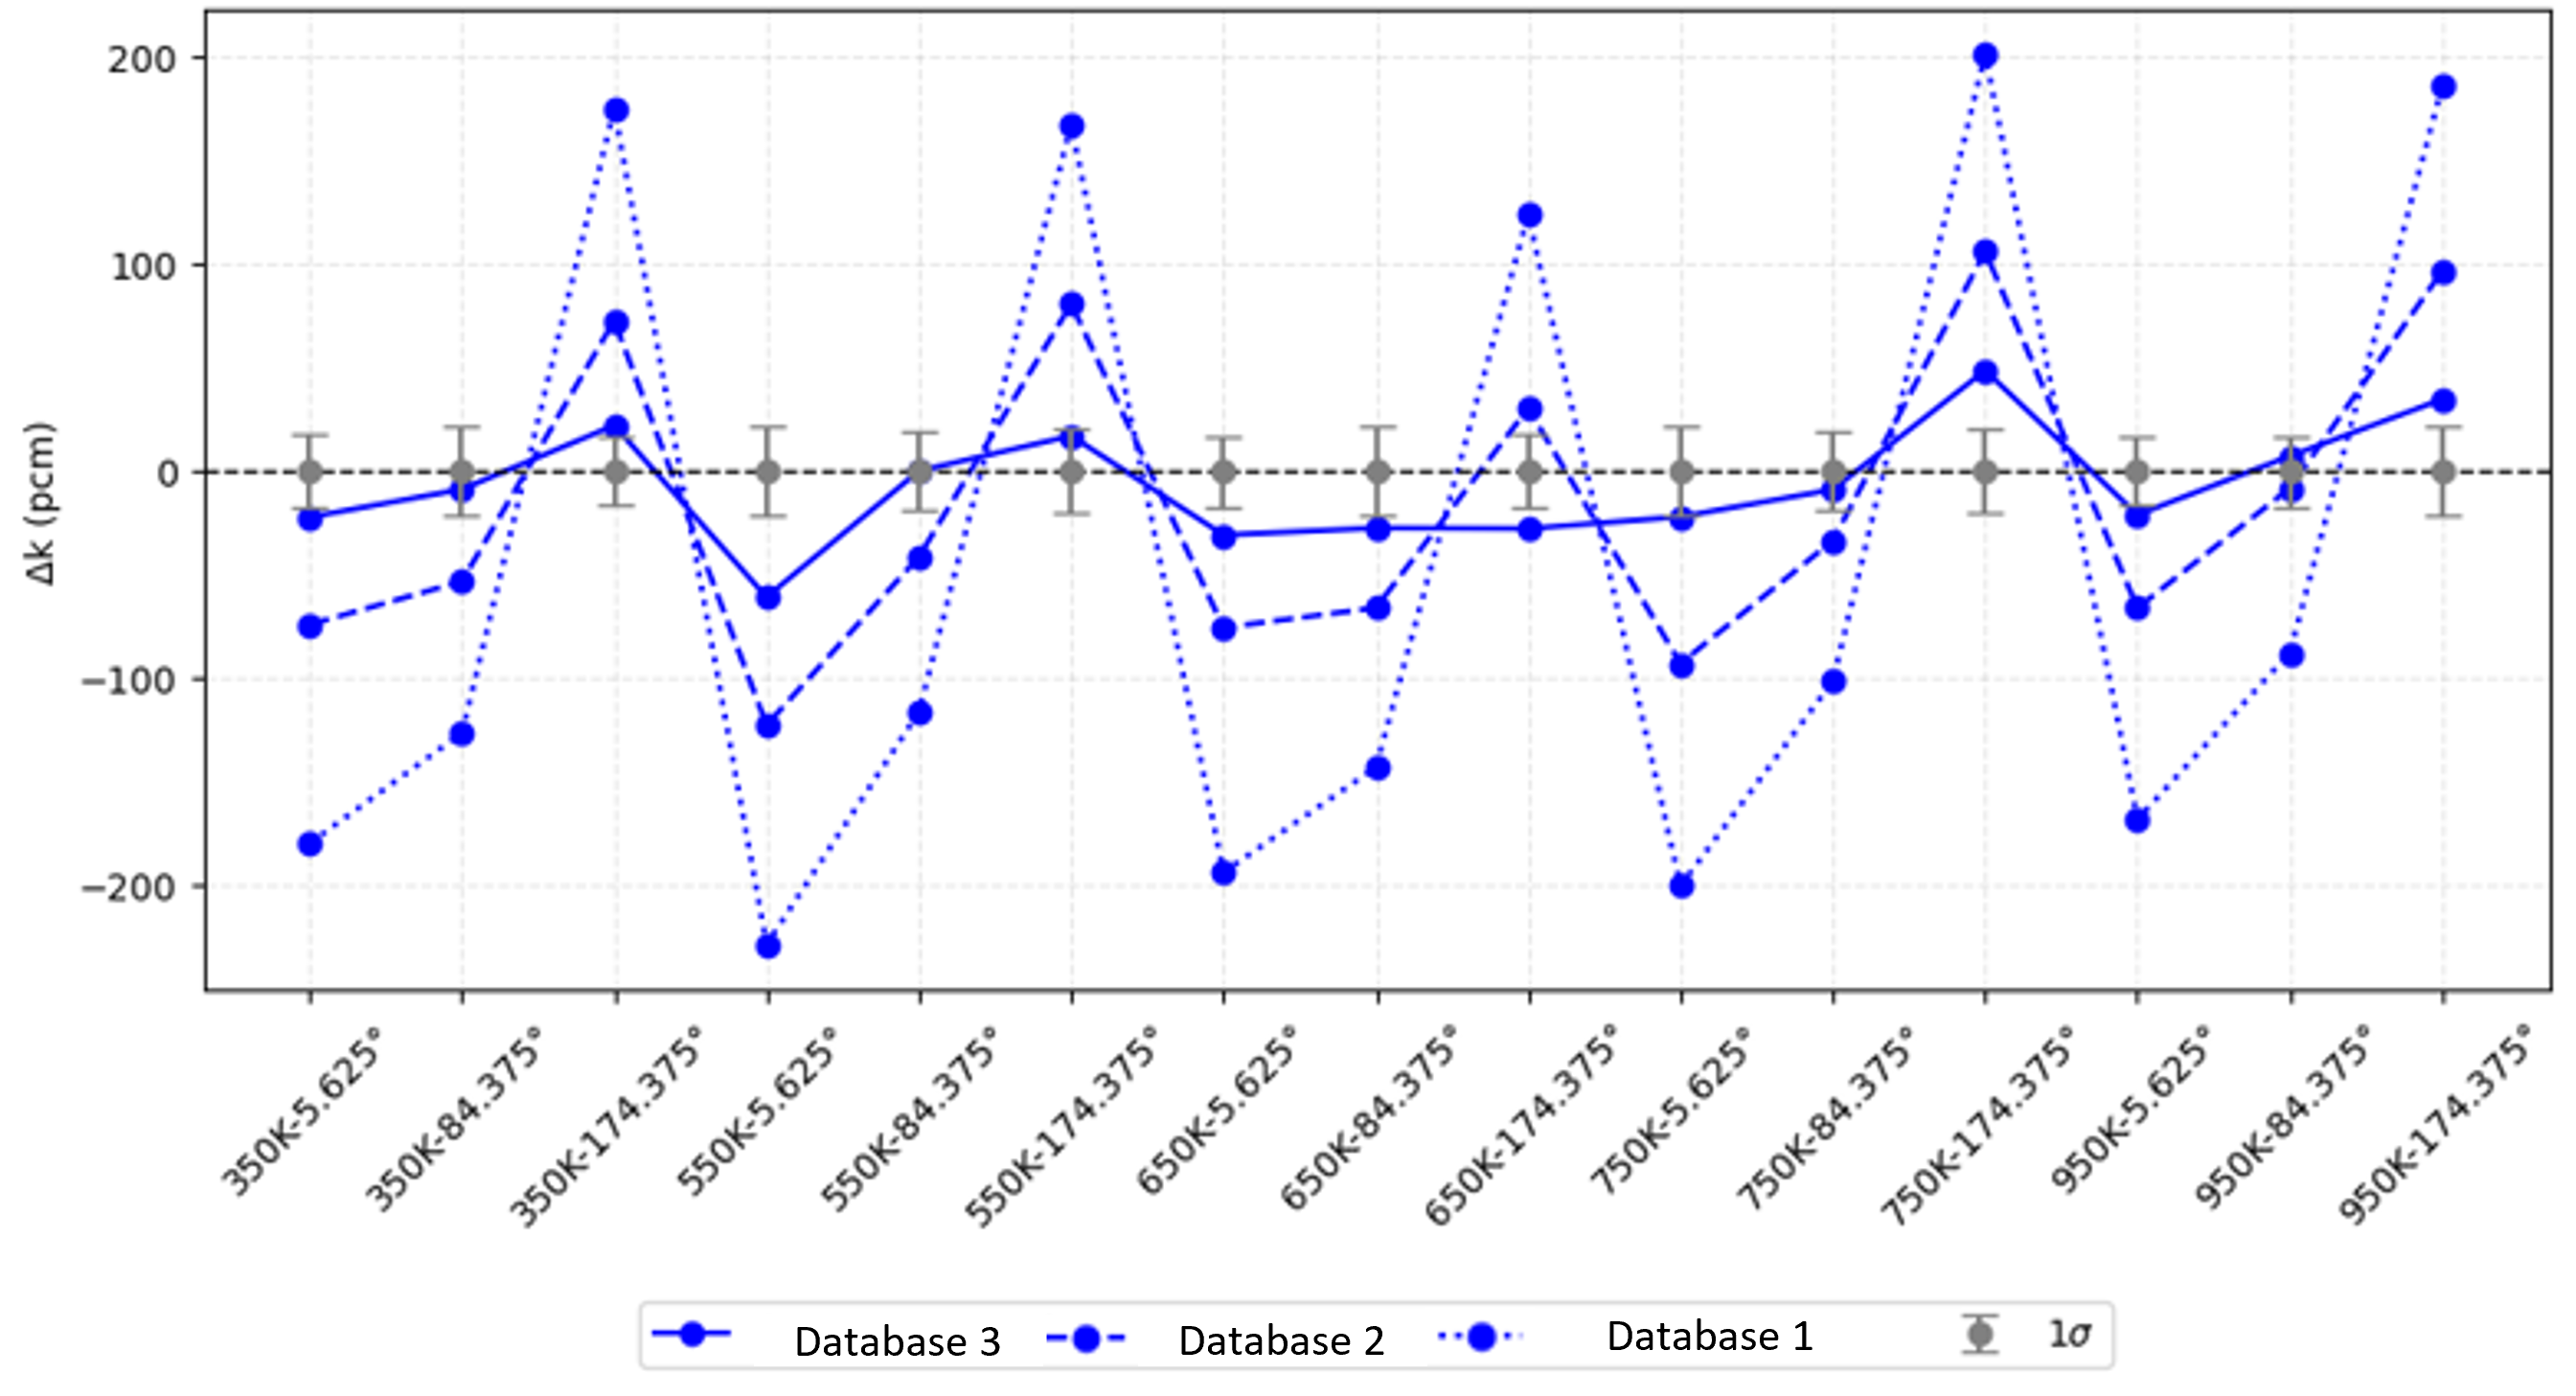
\includegraphics[scale=0.5]{images/linear_interpolation_improvement_changing_database.png}  % Modifica scale o usa width se serve
\caption{$\Delta k_{eff}$ using linear interpolation and varying the database.}
\label{fig:linear_interpolation_improvement_changing_database}
\end{figure}

\begin{table}[h!]
\centering
\caption{Interpolation errors for different databases using the linear method.}
\label{tab:table_delta_k_linear}
\begin{tabular}{lccccc}
\cline{2-6}
           & \multicolumn{3}{c}{$\Delta k_{eff}$ (pcm)} & RMSE - $\tilde{F}$ (\%)   & $max(\left|e \right|)$   \\ \cline{2-6} 
           & Min                & Max                & RMSE-${k_{eff}}$               &   -       & RMSE-$max(e)$             \\ \hline
Database 1 & 87.866             & 228.73             & 164.85             & 1.12 &  2.4              \\ \hline
Database 2 & 8.44               & 122.76             & 74.24              & 1.1  &  1.6            \\ \hline
Database 3 & 0.089              & 61.01              & 28.506             & 0.82 &  1.2                    \\ \hline

\end{tabular}
\end{table}

\subsection{Reflector Correction Ratio Tests}
 These simulations involve variations in both the temperature distribution and the CD positions.

The analyzed test cases are presented and described in \cref{tab:cases_testing_cases_for_gradient_T}. 
\begin{table}[h!]
\caption{Testing cases description based on the fuel assemblies temperature ($T_f$), reflector assemblies temperature ($T_r$) and the CD insertion angle ($\theta$).}
\centering
\begin{tabular}{llll}
\hline
       & $T_f$ & $T_r$ & $\theta$ \\ \hline
case 1 & 550 K  & 300 K  & 0°       \\ \hline
case 2 & 550 K  & 300 K  & 90°      \\ \hline
case 3 & 950 K  & 300 K  & 0°       \\ \hline
case 4 & 950 K  & 300 K  & 90°      \\ \hline
\end{tabular}
\label{tab:cases_testing_cases_for_gradient_T}
\end{table}


These four test cases are specifically designed to analyze the performance of the proposed RCR formulations under varying conditions of temperature gradients. By examining scenarios with different fuel temperatures ($T_f$), reflector temperatures ($T_r$), and CD rotation angle ($\theta$), we aim at comprehensively assessing how effective the correction ratio is. A temperature distribution sample of the case where $T_f \neq T_r$ is shown in \cref{fig:temperature_distribution_example_different_T_fuel_reflector}.
The selected cases also highlight how the accuracy decreases when no RCR is applied, particularly in configurations where the reflector temperature differs from that of the core.        

\begin{figure}[h!]
\centering

\includegraphics[scale=0.6]{images/grad_temp_core_reflector.png}  % Modifica scale o usa width se serve
\caption{Temperature distribution sample with different temperatures of the fuel (red) and reflector (blue).}
\label{fig:temperature_distribution_example_different_T_fuel_reflector}
\end{figure}


The results are reported in \cref{tab:cases_testing_cases_for_gradient_T2}, where $\Delta{k_{eff}}$, the maximum absolute value of $e$ and the RMSE are reported, applying the two definitions of the \rtwo{RCR}. In \cref{fig:Tf_550_Tr_300_4_plots} and \cref{fig:Tf_550_Tr_300_CD_90_4_plots} the results of Case 1 and Case 2 are reported. \rtwo{Each figure displays four panels: the reference fission source, the cell-wise combined uncertainty $\sigma_{tot,i}$ defined in \cref{subsec:Uncertainty}, and the local deviation $e_i$ of the uncorrected and of the corrected case, both expressed in units of that same uncertainty. The two deviation panels share the same colour scale, and the cells whose deviation does not exceed $2\sigma_{tot,i}$ are drawn as transparent outlines, so that only the statistically significant discrepancies remain visible. Only the corrected cases using \cref{eq:correction_ratio_2} are shown.} 

\begin{table}[h!]
\caption{Testing cases with different uniform $T_f$ and $T_r$ and CD position error. \rtwo{At $\theta = 0$ the two formulations of the RCR coincide, so for Cases 1 and 3 only the first one is reported.}}
\centering
\begin{tabular}{llcccc}
\cline{3-6}
&                                                  & Case 1 & Case 2 & Case 3 & Case 4 \\ \hline
$\sigma_{k_{eff}}$ (pcm)                                 & \multicolumn{1}{l|}{\rtwo{reference}}                      & \rtwo{18}     & \rtwo{18}     & \rtwo{19}     & \rtwo{18}     \\ \hline
\multirow{3}{*}{$\Delta k_{eff}$ (pcm)} & \multicolumn{1}{l|}{uncorrected}  & -111   & -176   & -352   & -415   \\
& \multicolumn{1}{l|}{\rtwo{RCR, \cref{eq:correction_ratio_1}}}         & \rtwo{33}     & -131   & 5      & -306   \\
& \multicolumn{1}{l|}{\rtwo{RCR, \cref{eq:correction_ratio_2}}}         & -     & -4      &  -     & 12     \\ \hline

\multirow{3}{*}{max($|e|$) (\%)} & \multicolumn{1}{l|}{uncorrected}     & \rtwo{3.7}    & \rtwo{3.6}    & \rtwo{7.5}    & \rtwo{8.3}    \\
& \multicolumn{1}{l|}{\rtwo{RCR, \cref{eq:correction_ratio_1}}}        & \rtwo{1.5}   & \rtwo{1.6}      & \rtwo{1.8}      & \rtwo{2.7}   \\
& \multicolumn{1}{l|}{\rtwo{RCR, \cref{eq:correction_ratio_2}}}        &  -    & \rtwo{1.7}   & -      & \rtwo{1.5}    \\ \hline

\multirow{3}{*}{RMSE-$\tilde{F}$ (\%)}  & \multicolumn{1}{l|}{uncorrected}  & \rtwo{1.7}     & \rtwo{1.9}    & \rtwo{4.4}    & \rtwo{4.7}    \\
& \multicolumn{1}{l|}{\rtwo{RCR, \cref{eq:correction_ratio_1}}}                   & \rtwo{0.48}    & \rtwo{0.53}   & \rtwo{0.48}    & 1.1   \\
& \multicolumn{1}{l|}{\rtwo{RCR, \cref{eq:correction_ratio_2}}}                   & -    & \rtwo{0.41}    & -    & \rtwo{0.60}    \\ \hline
\end{tabular}
\label{tab:cases_testing_cases_for_gradient_T2}
\end{table}


\begin{figure}[h!]
\centering
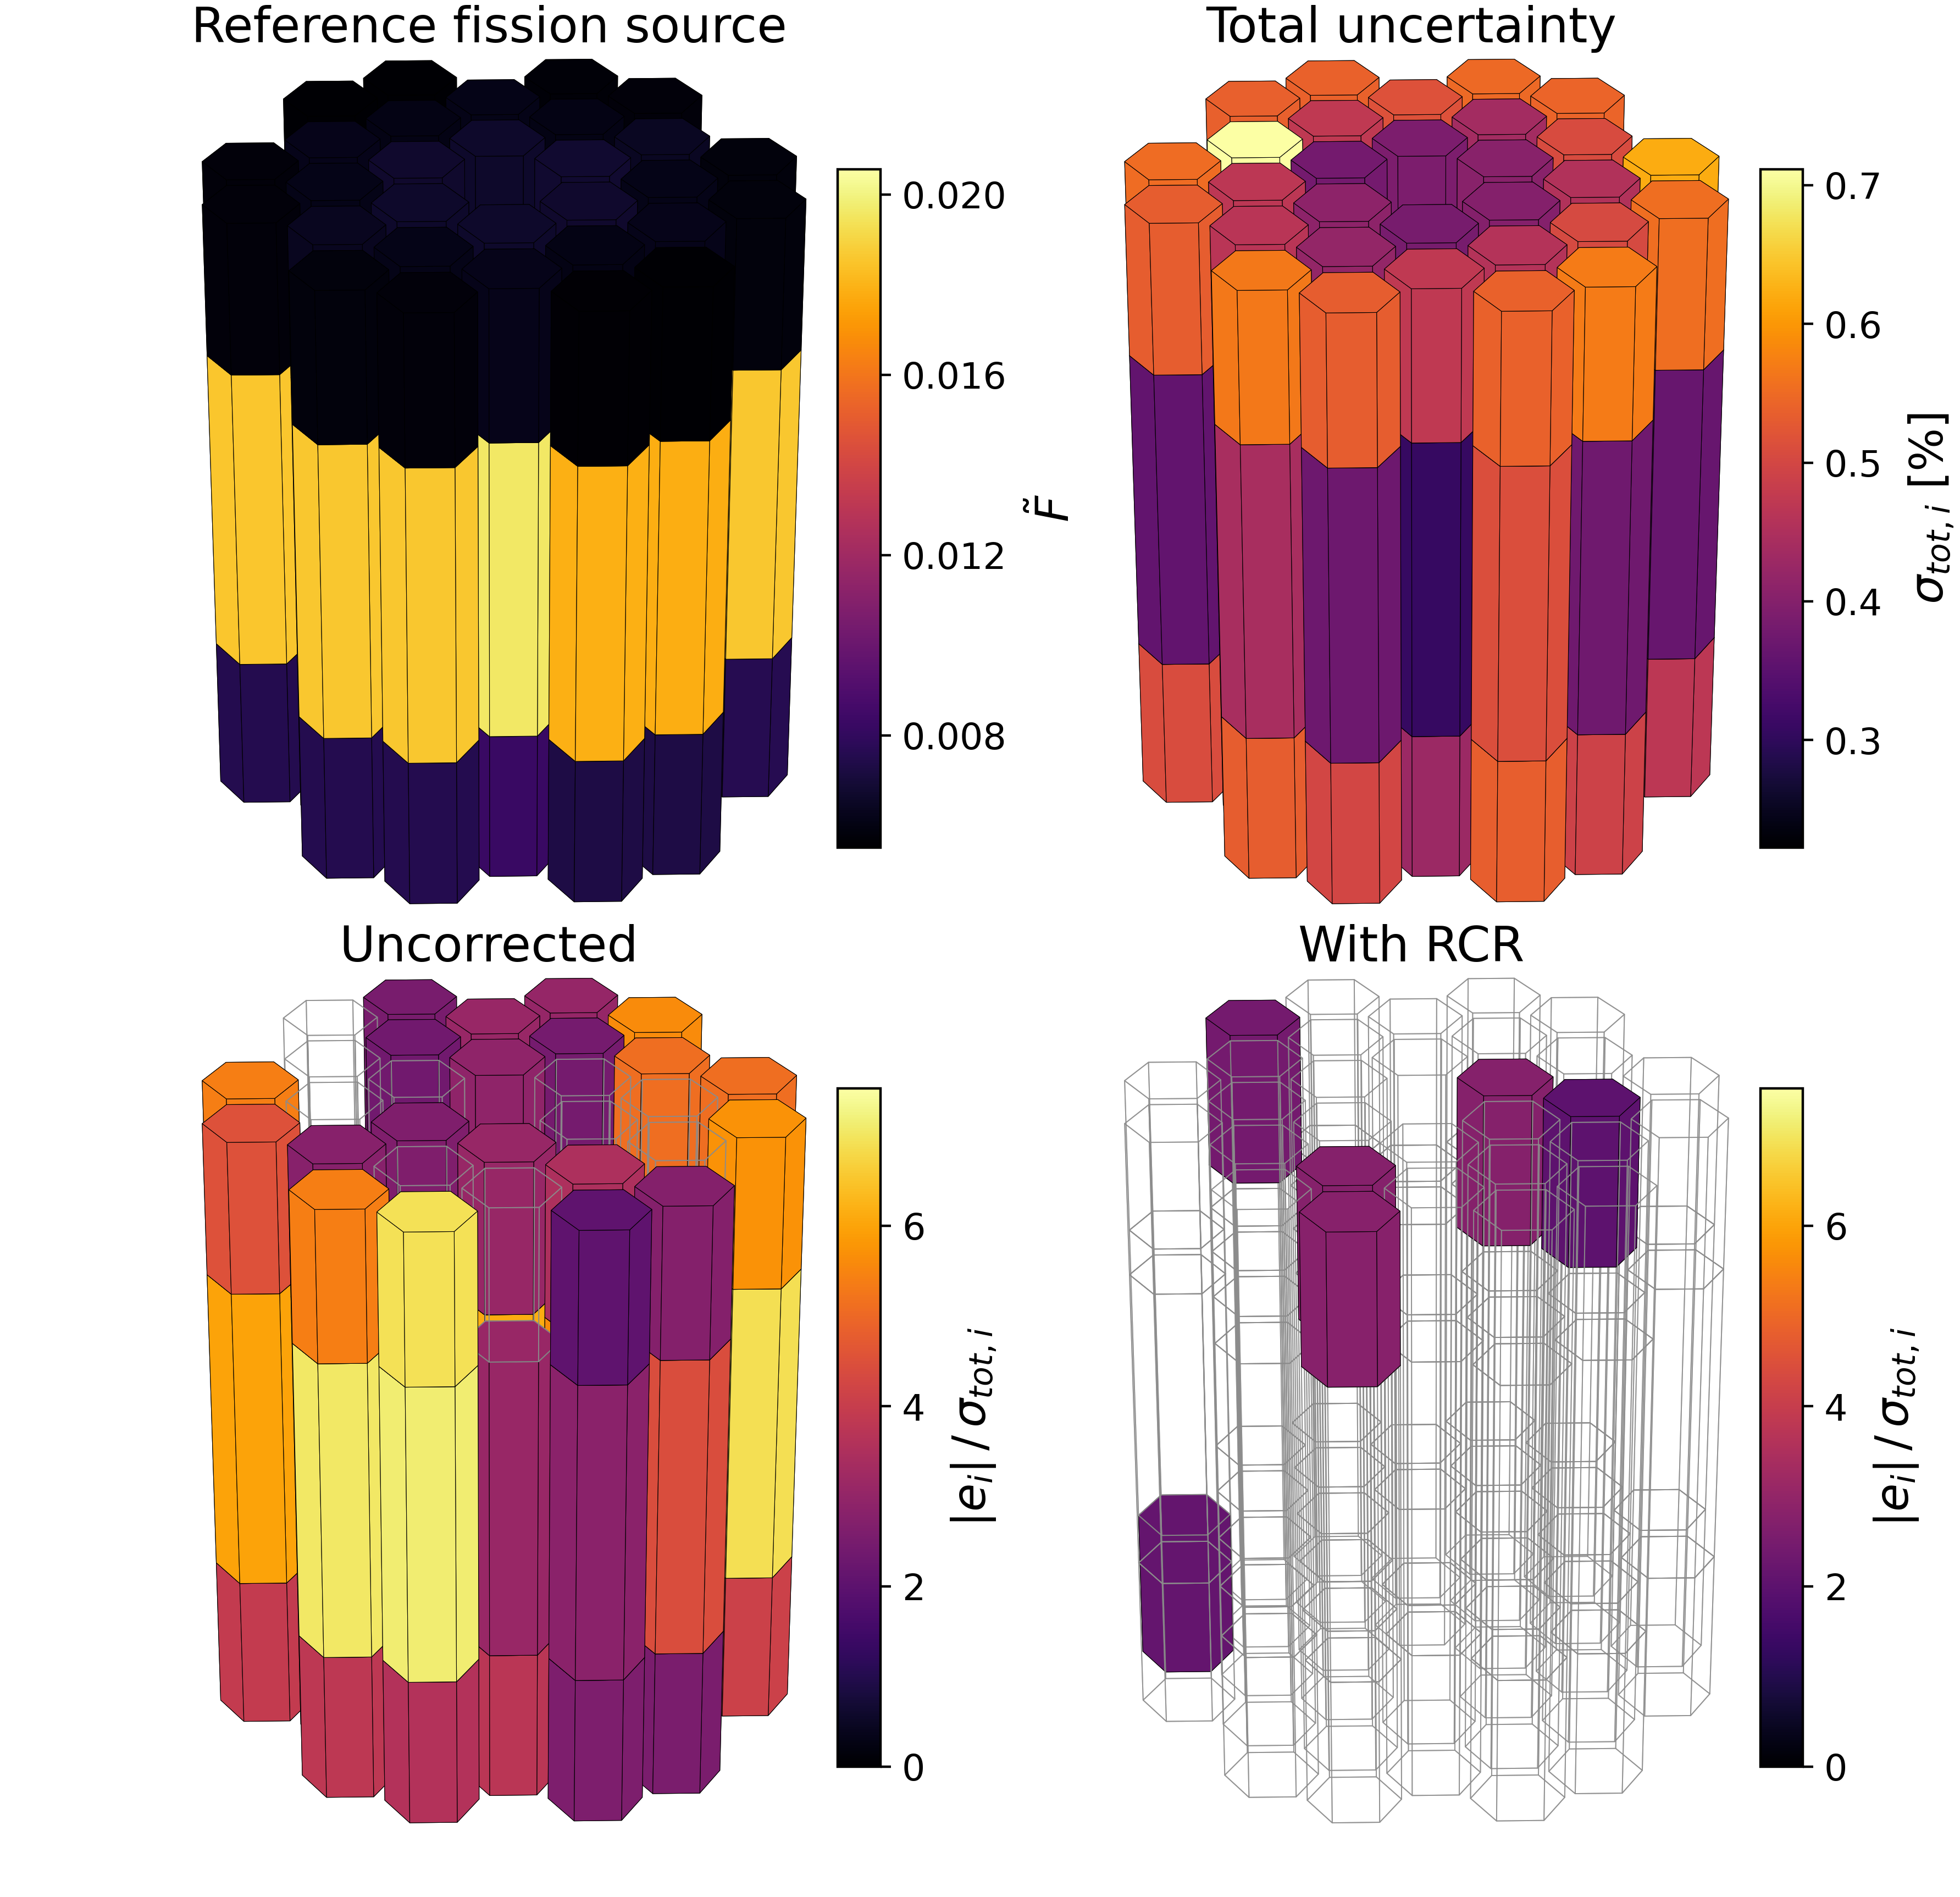
\includegraphics[scale=0.50]{images/Tf_550_Tr_300_4_plots.png}  % Modifica scale o usa width se serve
\caption{Case 1 of \cref{tab:cases_testing_cases_for_gradient_T}. The corrected case uses \cref{eq:correction_ratio_2}.}
\label{fig:Tf_550_Tr_300_4_plots}
\end{figure}

\begin{figure}[h!]
\centering
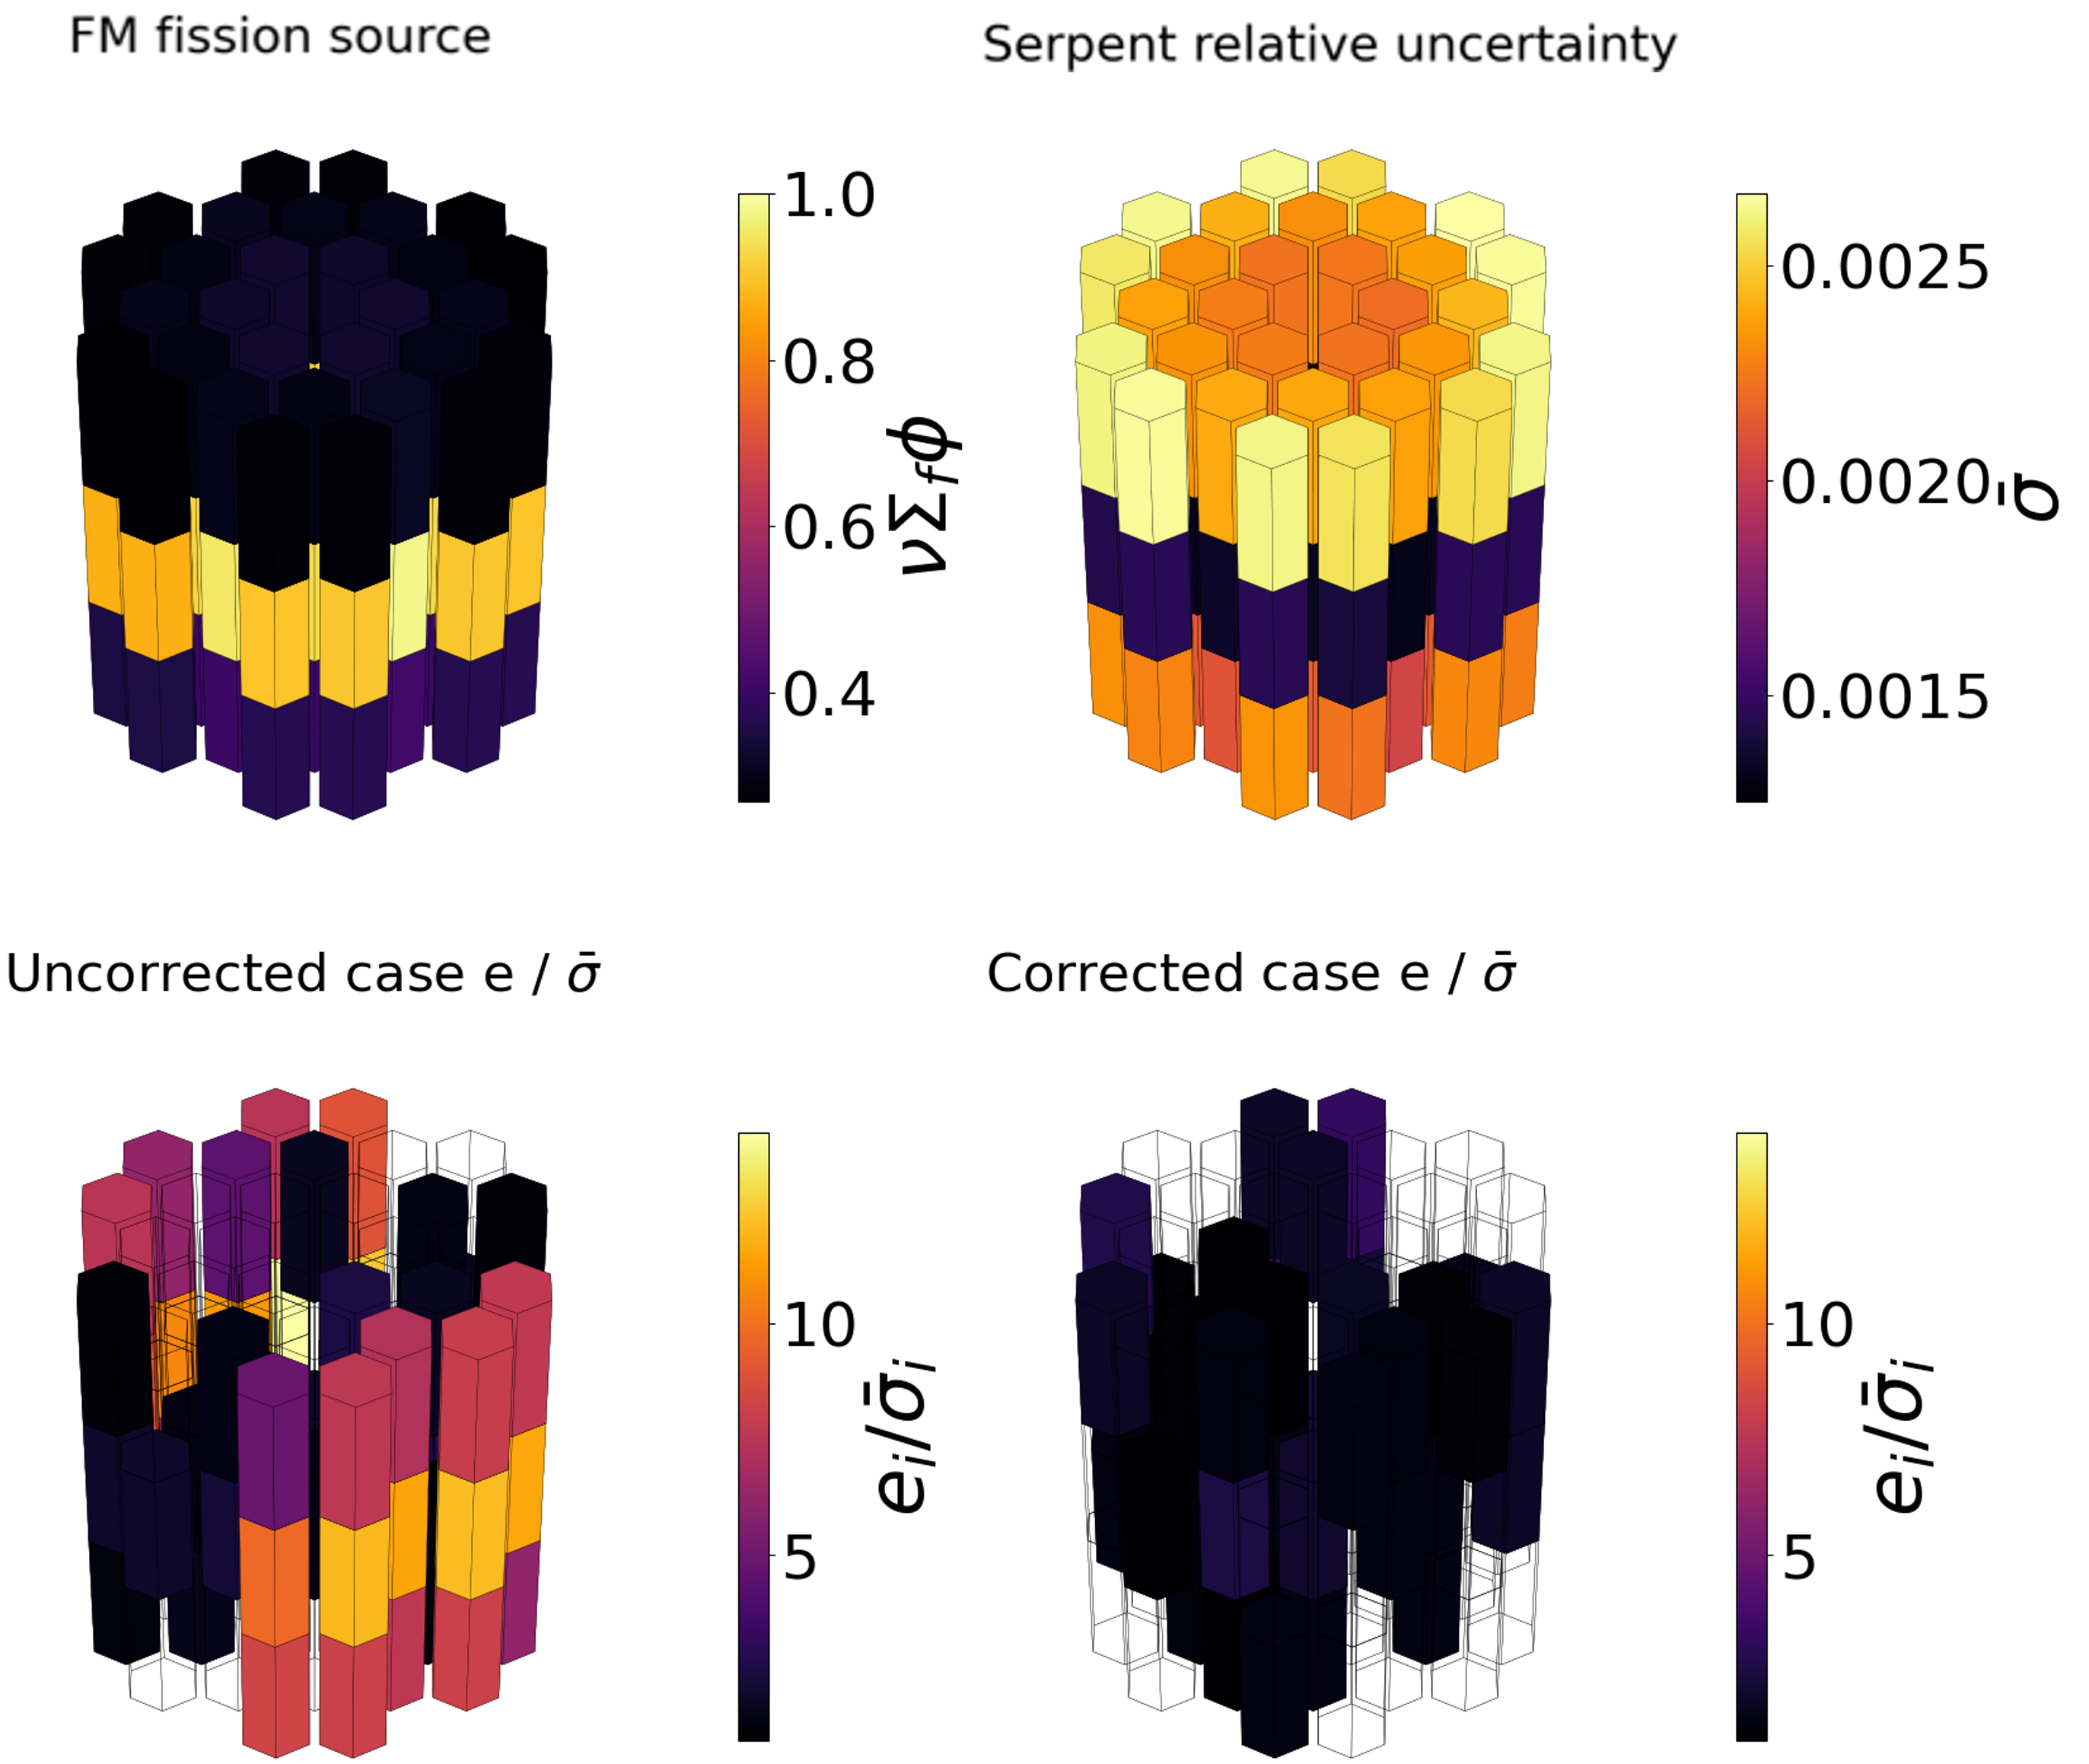
\includegraphics[scale=0.50]{images/Tf_550_Tr_300_CD_90_4_plots.png}  % Modifica scale o usa width se serve
\caption{Case 2 of \cref{tab:cases_testing_cases_for_gradient_T}. The corrected case uses \cref{eq:correction_ratio_2}.}
\label{fig:Tf_550_Tr_300_CD_90_4_plots}
\end{figure}

It can be observed that, in the uncorrected cases, the error in $k_{eff}$ is substantially larger than the statistical uncertainty of the reference cases, which is around 18 pcm, and it tends to increase with the temperature difference between the reflector and the active region. Using the RCR formulation given in \cref{eq:correction_ratio_1}, when the CDs are inserted into the system, the error is reduced compared to the uncorrected case. As a reminder, \cref{eq:correction_ratio_1} does not account for the combined effects of the reflector temperature gradient and CD positions. When the second RCR formulation (\cref{eq:correction_ratio_2}) is applied, the error further reduces and falls below the Serpent 2 statistical uncertainty.


\subsection{Core temperature distribution tests}
To analyze how the method performs when a non-uniform and non-symmetric temperature distribution is used, three more test cases are reported in the following. The first one (case 5) uses a non-uniform symmetric $T_f$ distribution, the second one (case 6) uses a non-uniform and non-symmetric distribution, while the third one (case 7) uses a realistic temperature distribution, calculated using \cref{eq:correction_power_temperature}. 
The temperature distributions of the three new cases are shown in \cref{fig:cases_5_6_7_temperature_distributions}. 


\begin{figure}[h!]
\centering
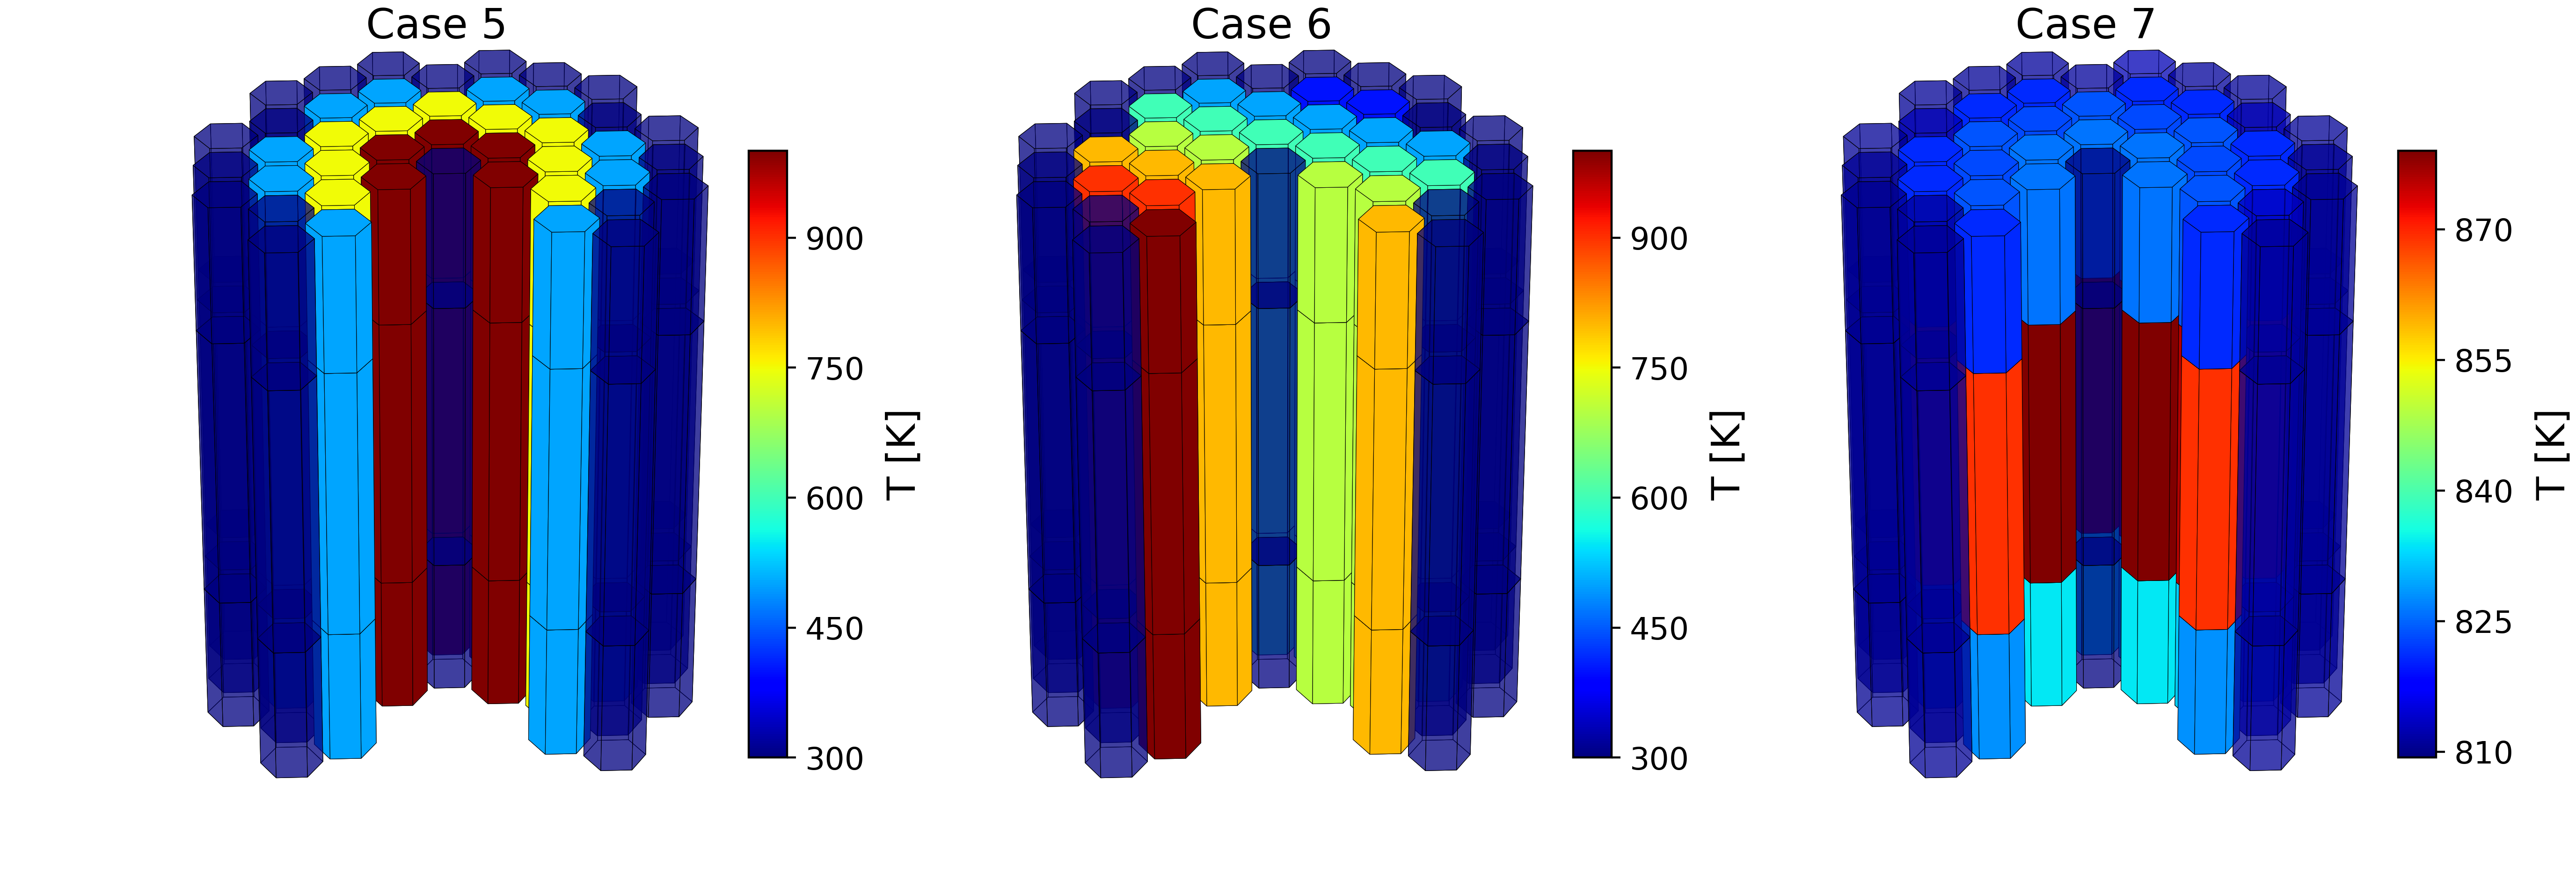
\includegraphics[scale=0.4]{images/cases_5_6_7_temperature_distributions.png}  % Modifica scale o usa width se serve
\caption{Temperature distributions of the fuel and reflector assemblies for Cases 5, 6 and 7. The assemblies of a sextant are removed to see the temperature of the innermost cells.}
\label{fig:cases_5_6_7_temperature_distributions}
\end{figure}

In Case 5, three different temperature values are defined over the three rings of fuel of the system. The temperature decreases from the center towards the outer ring. The reflector temperature is set to 300 K, the outer ring is 500 K, the middle one 750 K and the inner one 1000 K.
In Case 6, the temperature of the fuel increases linearly along the y-direction, starting from 350 K to 1000 K, while the reflector temperature is set to 300 K.
\rtwo{In Case 7 a more realistic condition is considered, in which the reflector is not isothermal but carries a temperature profile of its own. The fuel temperature follows a power-like distribution obtained from \cref{eq:correction_power_temperature}, and a temperature profile has been imposed by hand on the reflector regions, in a way consistent with the adjacent fuel temperatures, with the sole purpose of testing the method in a configuration closer to an operating condition. Both distributions are resolved over the three axial regions of the mesh. The resulting local temperature difference between fuel and reflector is small, +5 K on average, and changes sign across the core, ranging from $-33$ K to $+48$ K.} As described in \cref{subsec:Power and fuel temperature correlation}, the correlation requires the $\Delta T_{range}$ and $T_{f,min}$ parameters. Moreover, since the corresponding fission source of the temperature distribution is not known \textit{a priori}, the temperature has to be updated iteratively by changing the fission source distribution with the new one, obtained by the previous evaluated fuel temperature distribution. 
\rtwo{In Case 7 the power is considered equal to 2 MW, that is, the nominal power. The resulting fuel temperature ranges between 823 K and 874 K across the ninety cells, and the reflector profile spans the same interval. The order of magnitude of these values has been set on the basis of a high-fidelity simulation using the MOOSE suite of codes \cite{giudicelli2024moose} at nominal power with extracted CDs.} \linelabel{rl:fig9cite}\rtwo{That simulation is shown in \cref{fig:comparison_test_cases_wo_and_w_correction_ratio1}, together with its profile along a line crossing the active region and the reflector. The profile makes the temperature difference between the two regions evident, since the temperature drops at the core-reflector interface, and it is the feature that the correction ratio described in \cref{subsection:Core reflector treatment} is meant to reproduce.}

\begin{figure}[h!]
\FloatBarrier
\centering
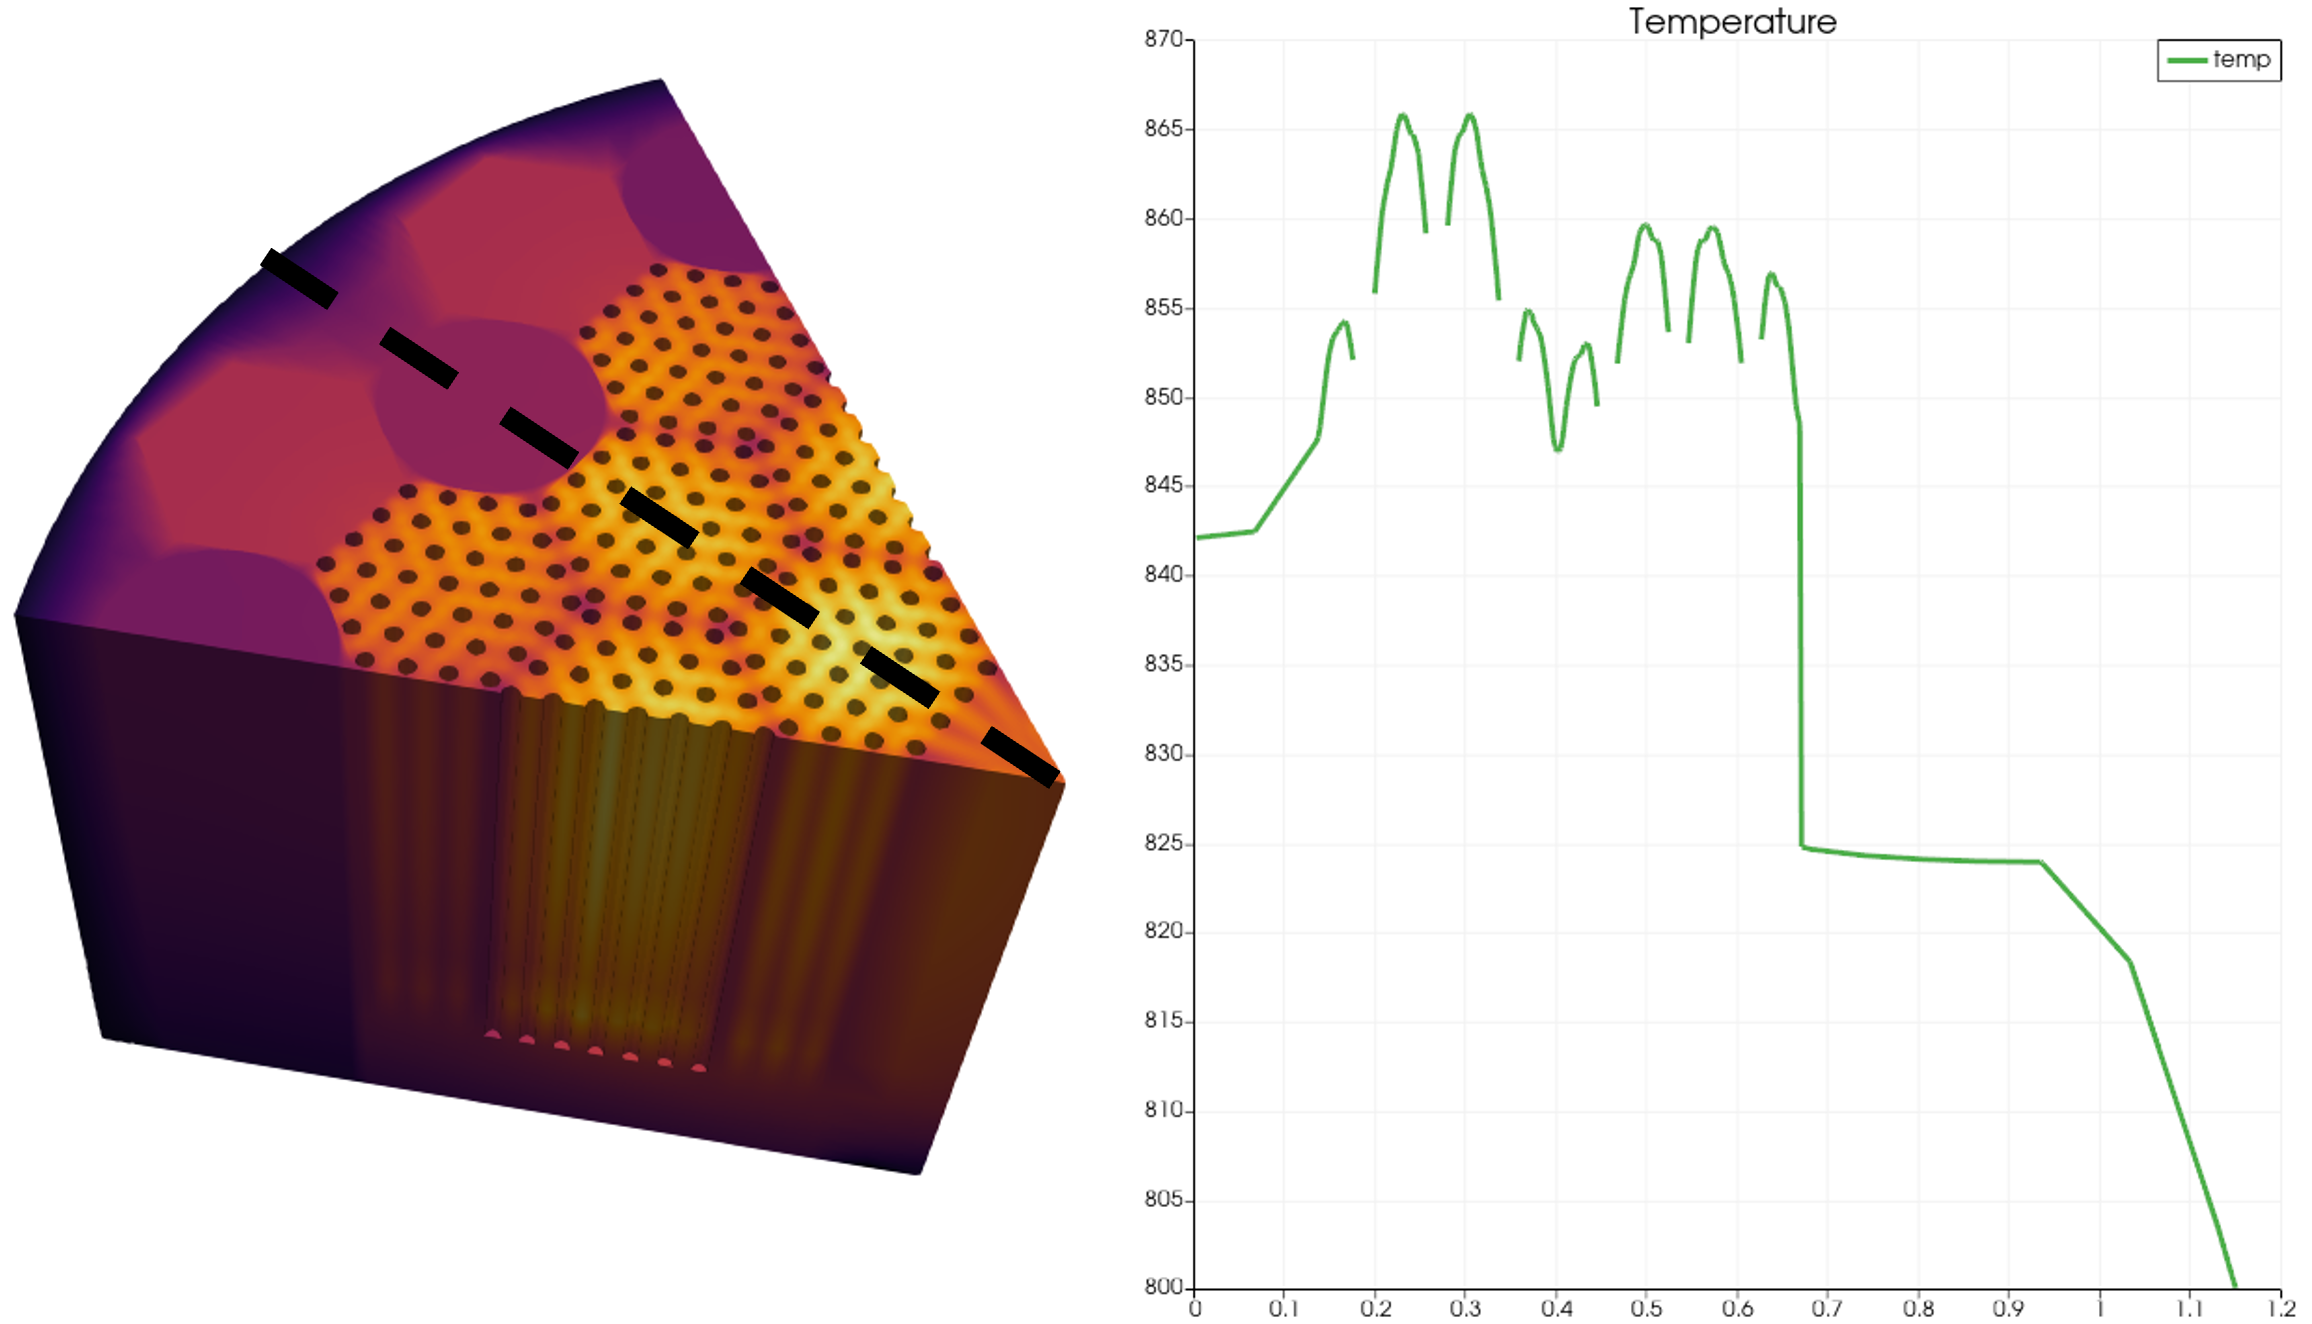
\includegraphics[scale=0.65]{images/realistic_temperature_desing_cenrtal_line_plot_horizontal.png}  % Modifica scale o usa width se serve
\caption{\rtwo{Temperature field of the HPMR obtained with a high-fidelity MOOSE simulation at nominal power with extracted CDs (left) and temperature profile along the dashed line crossing the active region and the reflector (right). The profile shows the temperature drop occurring at the core-reflector interface.}}
\label{fig:comparison_test_cases_wo_and_w_correction_ratio1}
\end{figure}

The results of these additional cases are reported in \cref{tab:testing_cases_5_6_7} and \cref{fig:Tf_rings_case_5,fig:Tf_linear_case_6,fig:Tf_power_like_case_7}. 
\rtwo{The FM method reproduces with acceptable accuracy even cases with strongly non-uniform temperature profiles such as Cases 5 and 6. The behaviour of the correction, however, is not the same in the three cases, and the difference is instructive. In Case 6, where the fuel temperature varies over 600 K along one direction while the reflector stays at 300 K, the correction removes almost the entire discrepancy on the multiplication factor, from $-201$ pcm to 9 pcm, and reduces the RMSE of the fission source from 3.0\% to 1.1\%. In Case 7 the local temperature difference between fuel and reflector is small and changes sign across the core, so there is little for the correction to recover, and indeed the corrected and uncorrected results are nearly indistinguishable. In Case 5 the correction reduces the deviation on the multiplication factor from $-100$ pcm to $-31$ pcm and the RMSE of the fission source from 3.4\% to 2.2\%. The improvement is appreciable but less pronounced than in Case 6, which is consistent with the nature of this case: the radial temperature profile is strongly non-uniform, with the innermost ring the hottest and the outermost the coldest, so that the local temperature difference varies steeply between adjacent rings while the correction is calibrated on a spatially uniform gradient. A zonation of the correction, in which the reference gradient matrix is generated separately for different regions of the core, is the natural way to address this and is left to future developments.}    

\begin{table}[h!]
\FloatBarrier
\caption{Results of the test cases using: ring-wise (Case 5), linear (Case 6) and power-like (Case 7) temperature distributions. Only the \cref{eq:correction_ratio_2} RCR formulation is applied.}
\centering
\begin{tabular}{llccc}
\cline{3-5}
&                                                  & Case 5 & Case 6 & Case 7 \\ \hline
$\sigma_{k_{eff}}$ (pcm) & \multicolumn{1}{l|}{\rtwo{reference}}         &    \rtwo{18}    &    \rtwo{19}    & \rtwo{19}       \\ \hline
\multirow{2}{*}{$\Delta k_{eff}$ (pcm)}   
& \multicolumn{1}{l|}{uncorrected}               &  \rtwo{-100}      & -201       &   \rtwo{-32}     \\
& \multicolumn{1}{l|}{\rtwo{RCR, \cref{eq:correction_ratio_2}}}    &   \rtwo{-31}     &  \rtwo{9}      &     \rtwo{-26}   \\ \hline
\multirow{2}{*}{max($|e|$) (\%)}     
& \multicolumn{1}{l|}{uncorrected}               &    \rtwo{5.9}    &   \rtwo{7.6}     &    \rtwo{1.2}    \\
& \multicolumn{1}{l|}{\rtwo{RCR, \cref{eq:correction_ratio_2}}}    &    \rtwo{5.1}   &   \rtwo{2.9}     &     \rtwo{1.2}   \\ \hline
\multirow{2}{*}{RMSE-$\tilde{F}$ (\%)}         
& \multicolumn{1}{l|}{uncorrected}               &     \rtwo{3.4}   &   \rtwo{3.0}  &   \rtwo{0.5}     \\
& \multicolumn{1}{l|}{\rtwo{RCR, \cref{eq:correction_ratio_2}}}    &      \rtwo{2.2}  &   \rtwo{1.1}   &   \rtwo{0.5}     \\ \hline
\end{tabular}
\label{tab:testing_cases_5_6_7}
\end{table}


\begin{figure}[h!]
\FloatBarrier
\centering
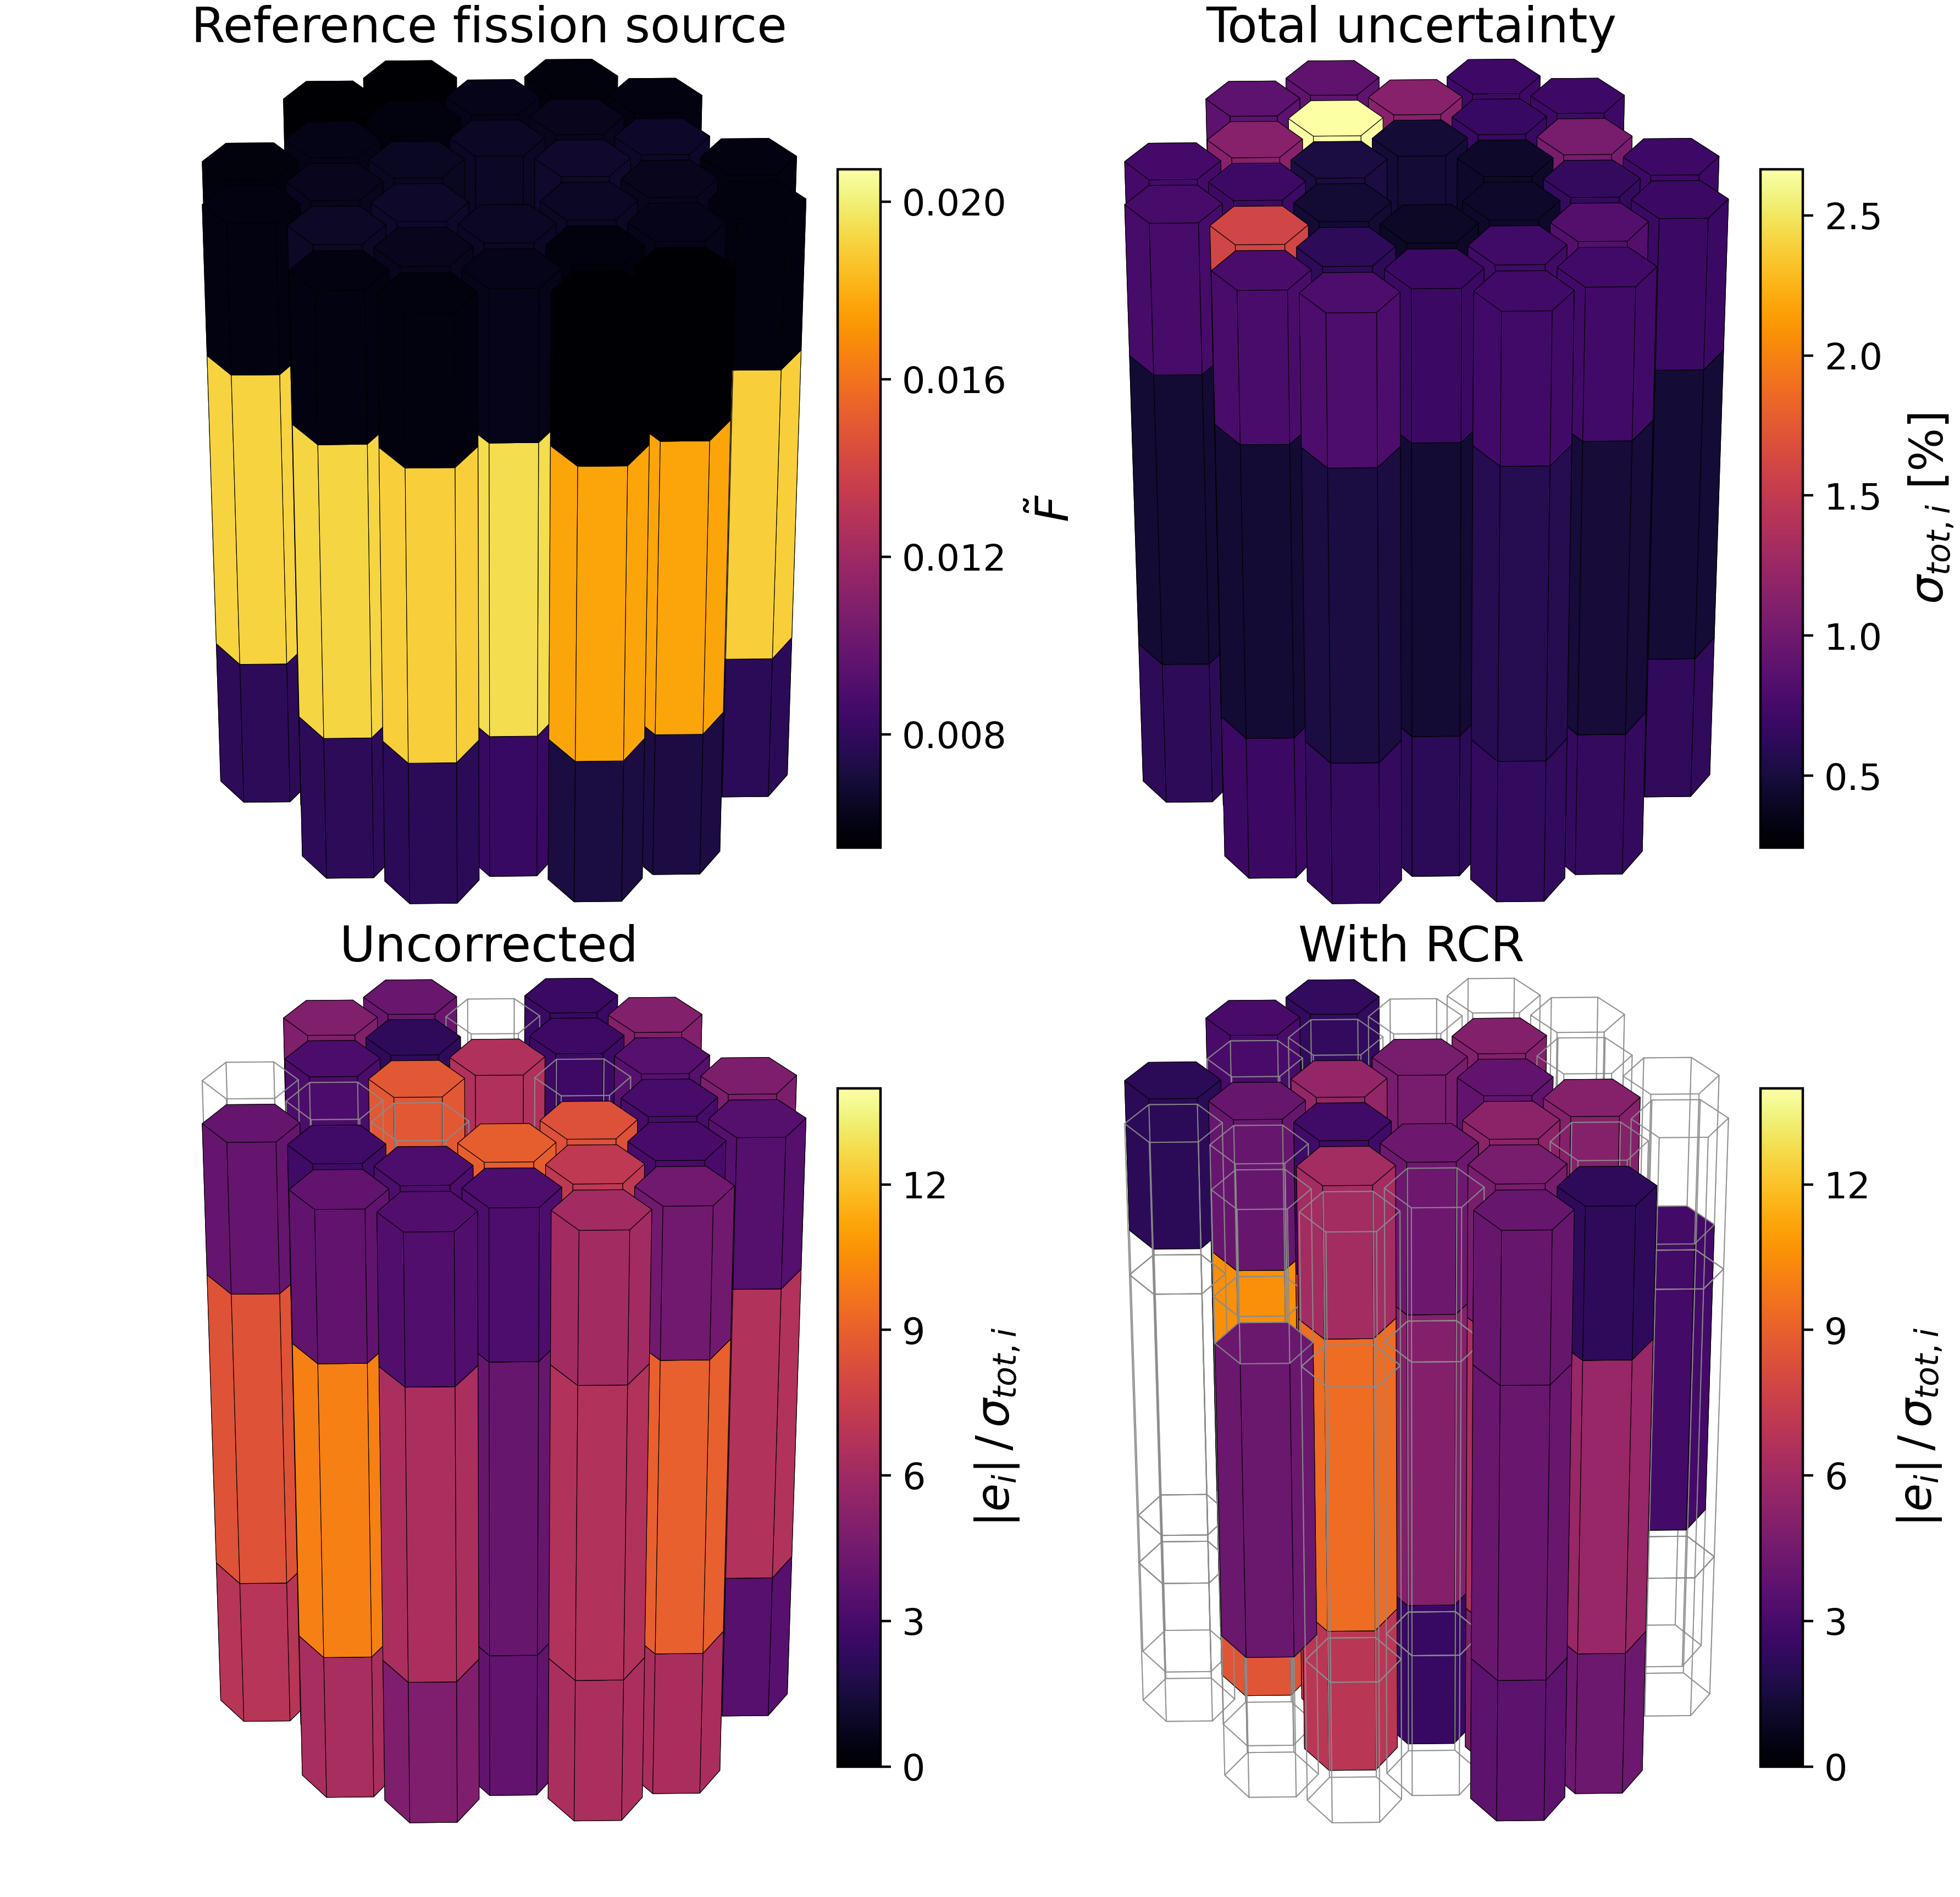
\includegraphics[scale=0.5]{images/Tf_rings_case_5.png}  % Modifica scale o usa width se serve
\caption{Case 5 of \cref{tab:testing_cases_5_6_7}. The corrected case uses \cref{eq:correction_ratio_2}.}
\label{fig:Tf_rings_case_5}
\end{figure}

\begin{figure}[h!]
\FloatBarrier
\centering
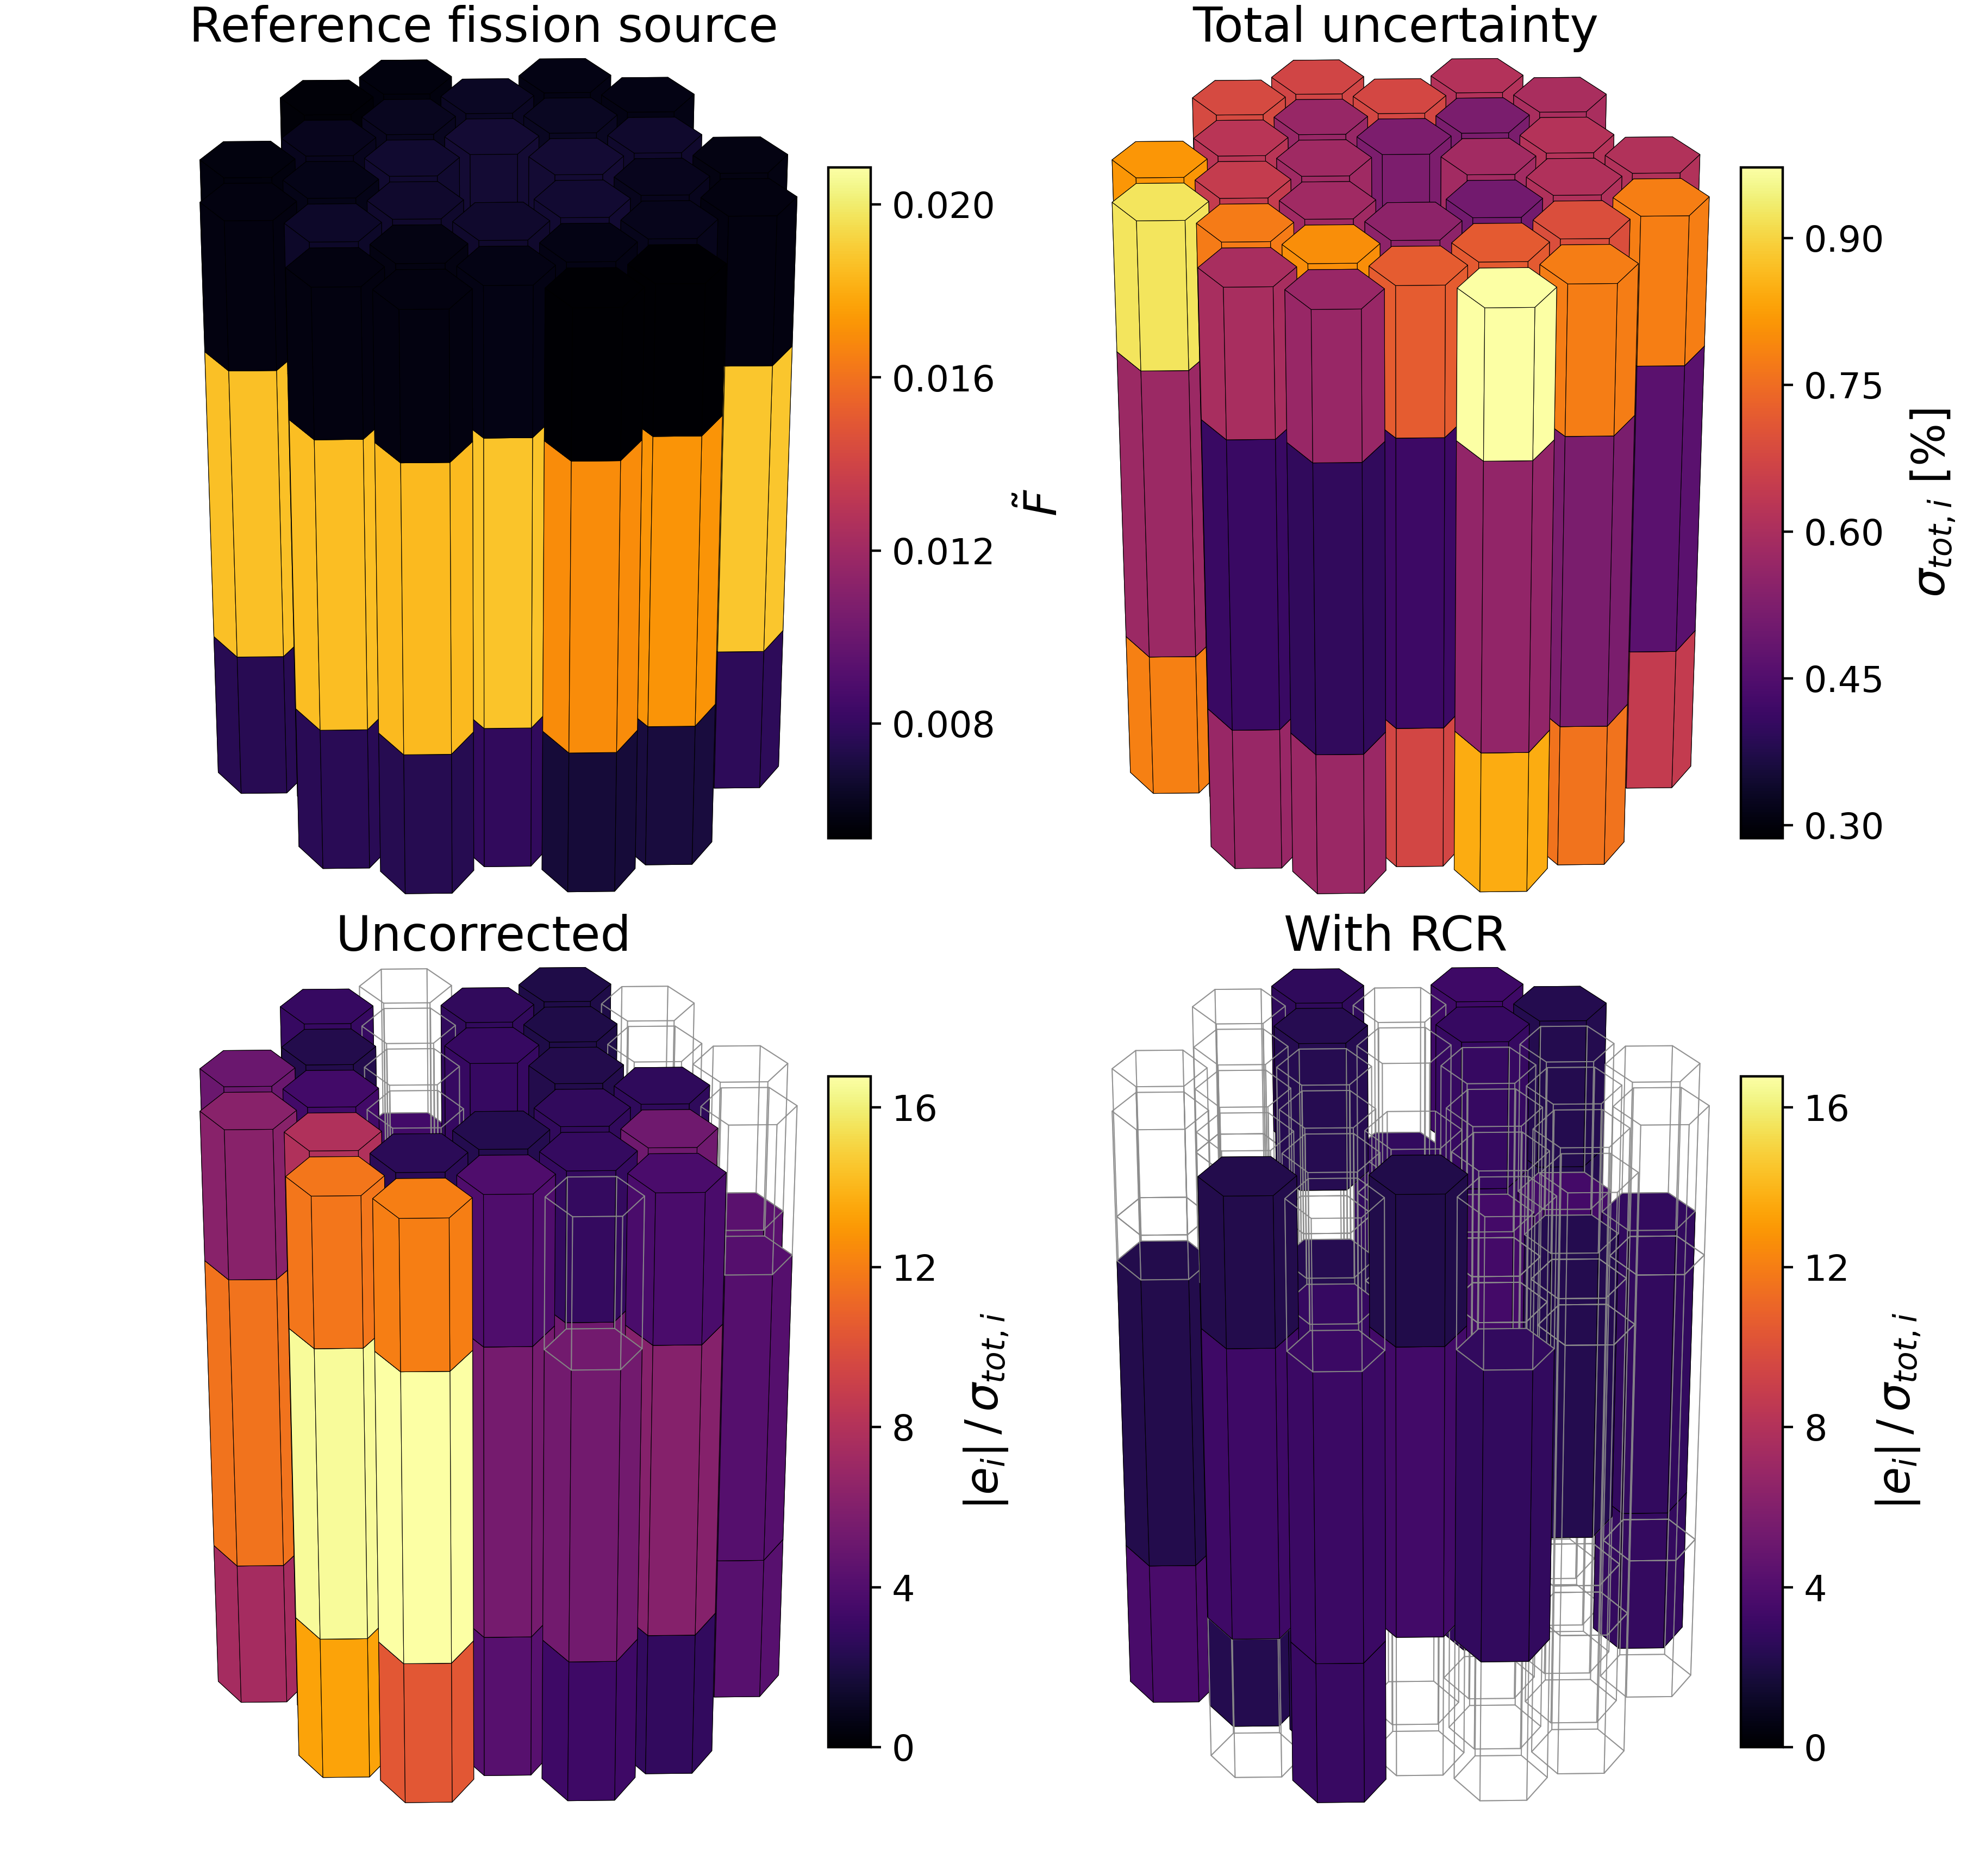
\includegraphics[scale=0.5]{images/Tf_linear_case_6.png}  % Modifica scale o usa width se serve
\caption{Case 6 of \cref{tab:testing_cases_5_6_7}. The corrected case uses \cref{eq:correction_ratio_2}.}
\label{fig:Tf_linear_case_6}
\end{figure}

\begin{figure}[h!]
\FloatBarrier
\centering
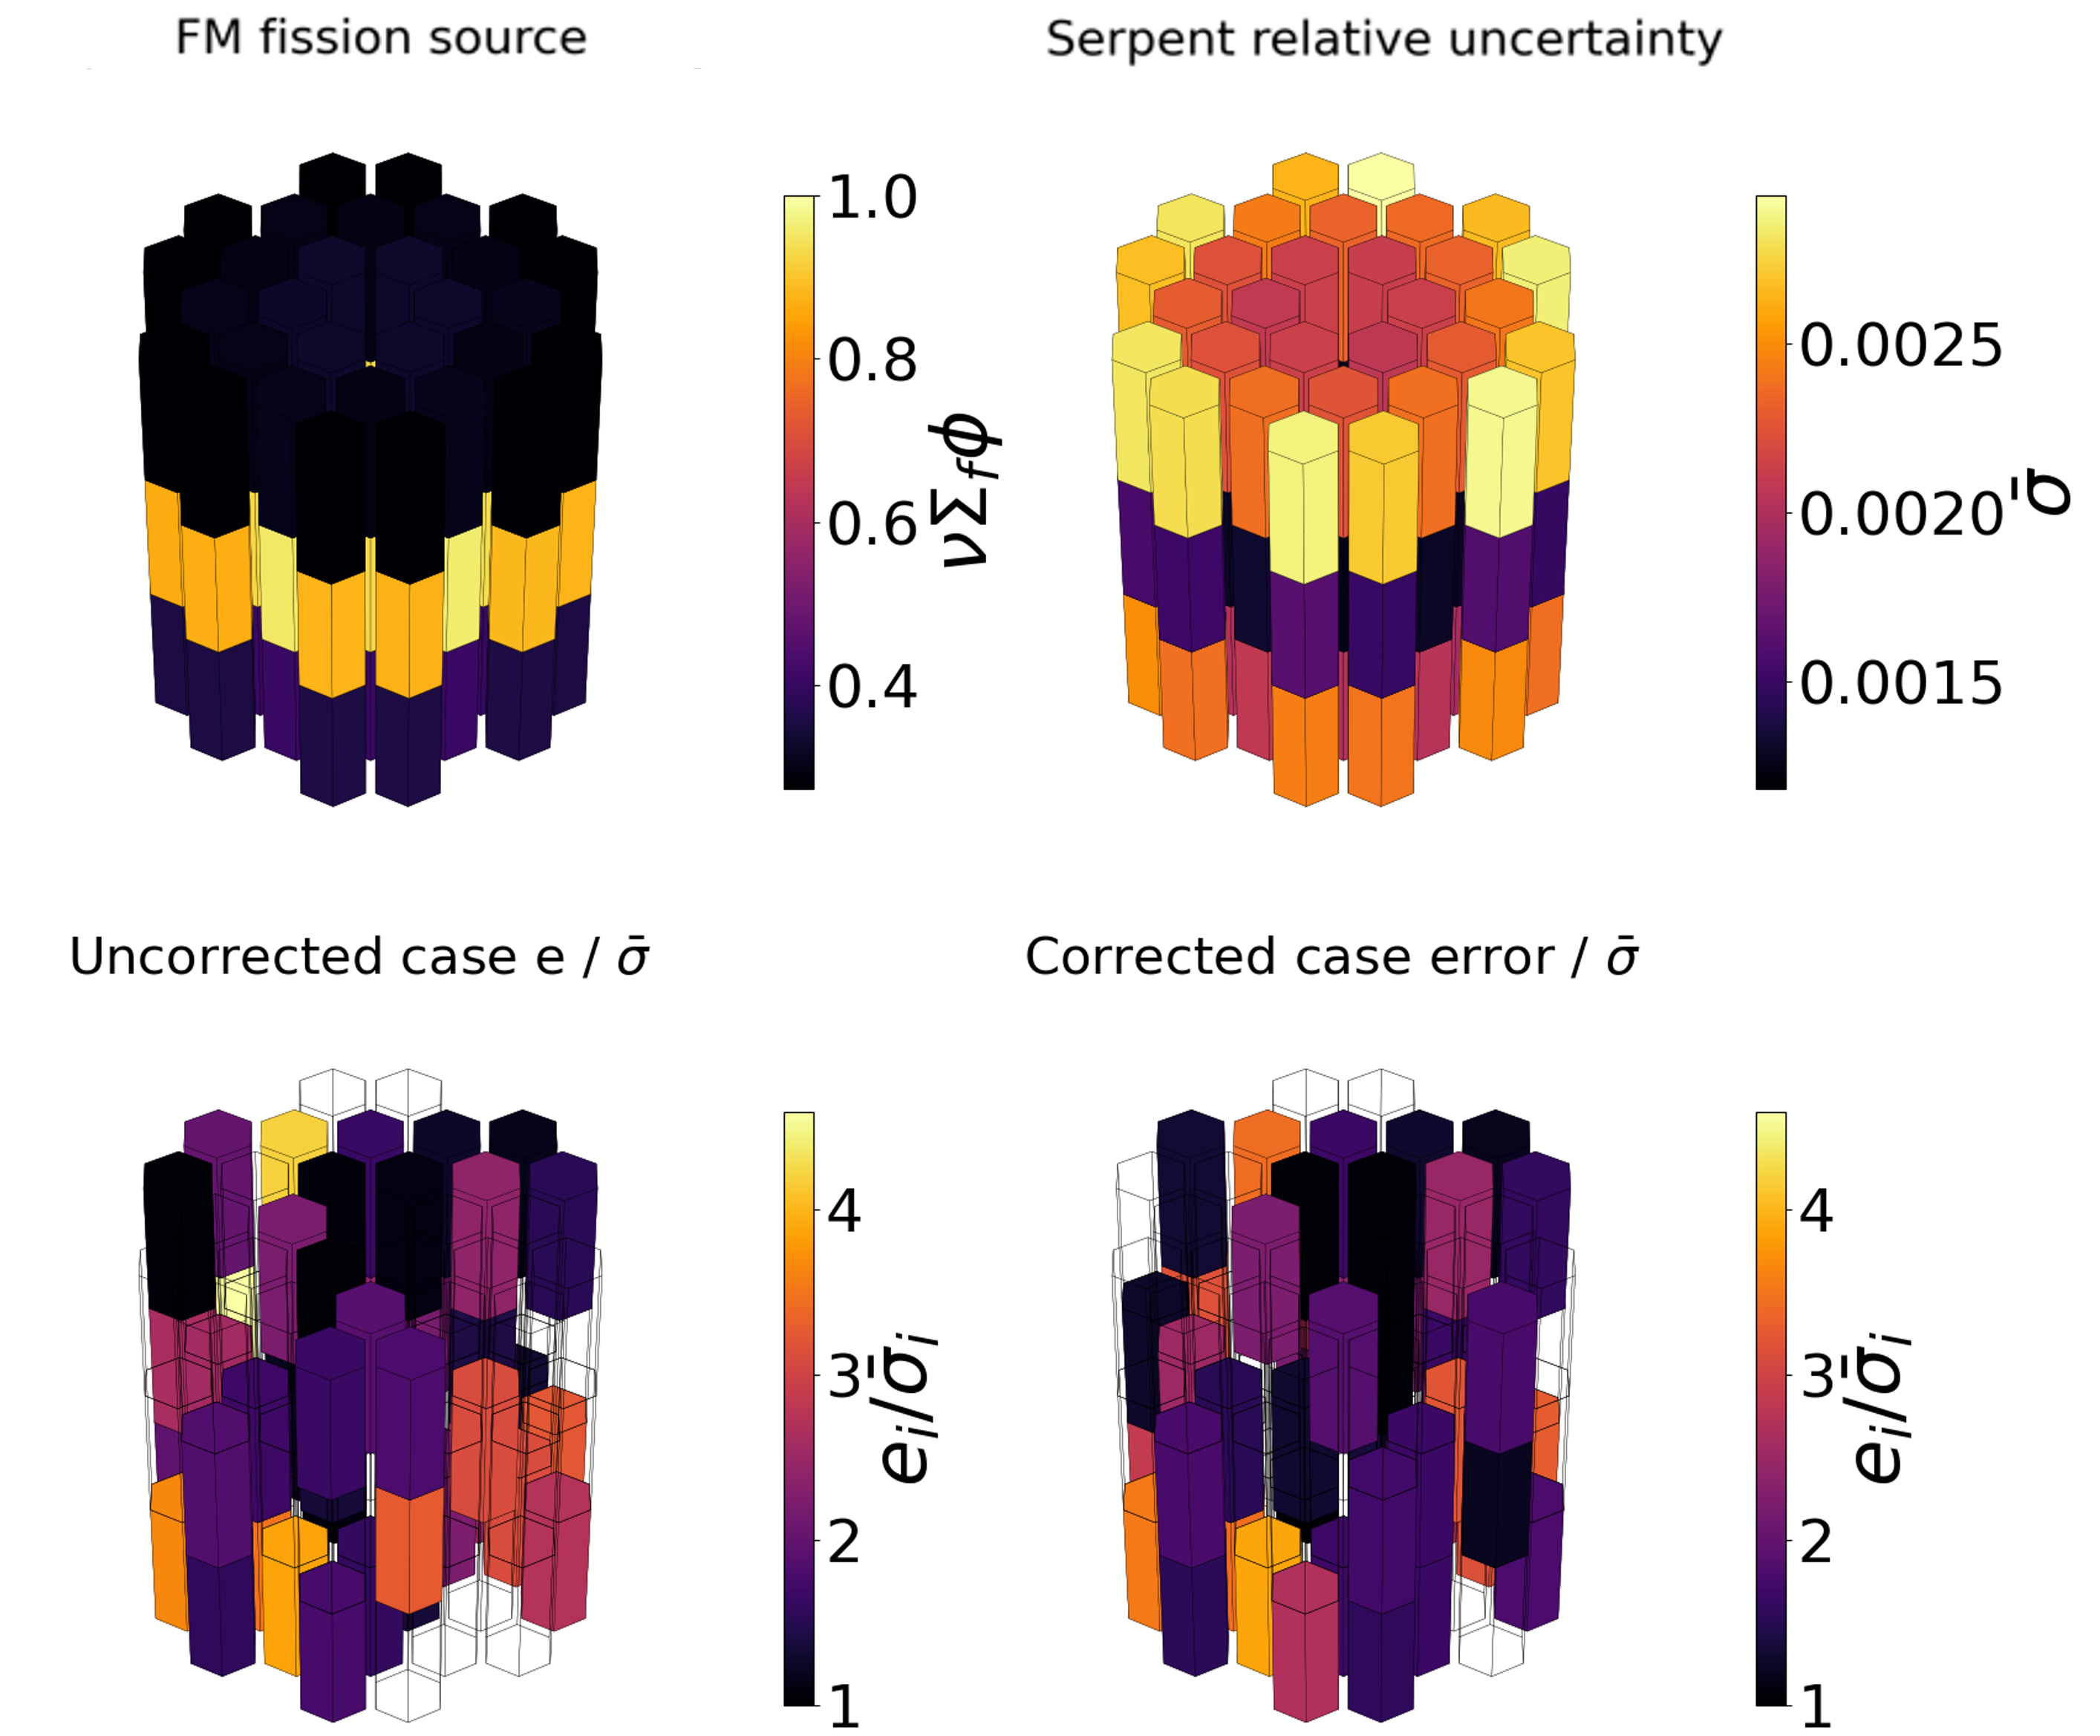
\includegraphics[scale=0.5]{images/Tf_power_like_case_7.png}  % Modifica scale o usa width se serve
\caption{Case 7 of \cref{tab:testing_cases_5_6_7}. The corrected case uses \cref{eq:correction_ratio_2}.}
\label{fig:Tf_power_like_case_7}
\end{figure}


\begingroup\rtwocolor
\subsection{Statistical significance of the residual discrepancies}
\label{subsec:UncertaintyBudget}
The seven test cases discussed so far are now used to quantify the statistical noise against which the residual discrepancies have to be judged, following the procedure described in \cref{subsec:Uncertainty}. The resulting budget is reported in \cref{tab:uncertainty_budget}.

\begin{table}[h!]
\FloatBarrier
\caption{\rtwo{Uncertainty budget of the interpolated results. $\sigma_{k}$ refers to the multiplication factor, $\sigma_{\tilde{F}}$ to the fission source, averaged over the ninety cells. The two contributions --- from the reference case (ref), and from the database (DB)  --- are combined in $\sigma_{tot}$, and for the fission source the combination is performed cell by cell and then averaged.}}
\centering
\begin{tabular}{lcccccc}
\hline
 & $\sigma_{ref,k}$ & $\sigma_{DB,k}$  & $\sigma_{tot,k}$ & $\sigma_{ref,\tilde{F}}$ & $\sigma_{DB,\tilde{F}}$ & $\sigma_{tot,\tilde{F}}$  \\
 & (pcm) & (pcm) & (pcm) & (\%) & (\%) & (\%) \\ \hline
Case 1 & 18 & 21 & 28 & 0.20 & 0.38 & 0.43 \\
Case 2 & 18 & 21 & 27 & 0.21 & 0.37 & 0.42 \\
Case 3 & 19 & 28 & 34 & 0.20 & 0.53 & 0.56 \\
Case 4 & 18 & 27 & 32 & 0.20 & 0.51 & 0.56 \\
Case 5 & 18 & 27 & 32 & 0.20 & 0.53 & 0.57 \\
Case 6 & 19 & 32 & 37 & 0.20 & 0.55 & 0.59 \\
Case 7 & 19 & 17 & 25 & 0.20 & 0.28 & 0.35 \\ \hline
\end{tabular}
\label{tab:uncertainty_budget}
\end{table}

The contribution of the database is comparable to, and on the fission source larger than, that of the reference calculation, so neither of the two can be neglected when judging the significance of a residual discrepancy. Using the combined values, the deviations obtained with the RCR of \cref{eq:correction_ratio_2} remain within about 1.2 combined standard deviations of the reference in all the seven cases, and, with the exception of Case 5, the RMSE of the fission source is of the same order as the combined noise. The local deviations reported in the figures of \cref{section:Results and discussion} are expressed in units of this combined uncertainty.
\endgroup

\subsection{Criticality search algorithm testing}
 Exploiting the good accuracy and the computational efficiency of the FM method, a criticality search algorithm based on the FM method is defined as described in \cref{subsec:criticality_search_method}, as proposed in \cite{Topham2020}. 

The power is provided as an input to \cref{eq:correction_power_temperature}, where the parameters used to determine the temperature distribution are the same as in Case 7. 
As it can be observed in \Cref{fig:critical_CD_angle_VS_power}, the relation between the critical CDs angle and the power is linear. This effect is attributable to the fact that the thermal feedback effect is smaller than the CD worth.
  

\begin{figure}[h!]
\FloatBarrier
\centering
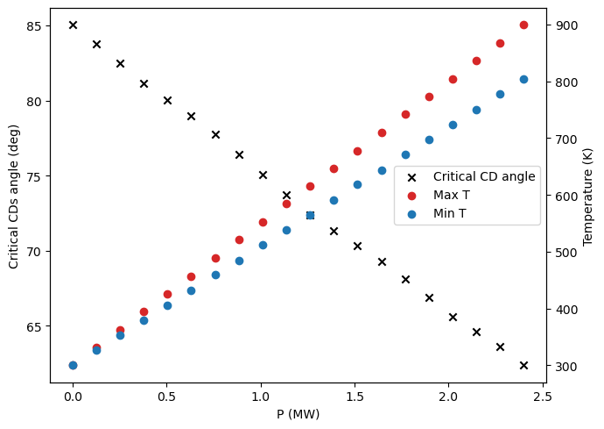
\includegraphics[scale=0.6]{images/critical_CD_angle_VS_power.png}  % Modifica scale o usa width se serve
\caption{Critical CDs angle at different reactor powers between 0 MW and 2.4 MW (black crosses). The blue and red dots represent the minimum and maximum temperature of the system at the corresponding power, respectively.}
\label{fig:critical_CD_angle_VS_power}
\end{figure}

To verify if the critical CD angle calculated by the FM algorithm is accurate, four additional test cases are considered, at power levels: 0 MW, 0.8 MW, 1.6 MW, 2.4 MW. These cases are compared to reference Serpent 2 calculations. The results are reported in \cref{tab:testing_cases_8_9_10_11}.

\begin{table}[h!]
\FloatBarrier
\caption{Test cases at power levels 0 MW (Case 8), 0.8 MW (Case 9), 1.6 MW (Case 10), 2.4 MW (Case 11).}
\centering
\begin{tabular}{llcccc}
\cline{3-6}
&                                                  & Case 8 & Case 9 & Case 10 & Case 11 \\ \hline
$\sigma_{k_{eff}}$ (pcm) & \multicolumn{1}{l|}{\rtwo{reference}}         &    16    &    19    & 15  & 17    \\ \hline
$\Delta k_{eff}$ (pcm)   
& \multicolumn{1}{l|}{\rtwo{RCR, \cref{eq:correction_ratio_2}}}      &    23    &    38    & 19  & -20  \\ \hline
max($|e|$) (\%)     
& \multicolumn{1}{l|}{\rtwo{RCR, \cref{eq:correction_ratio_2}}}    &    0.8   &   1.2     &     1.4   & 2.2 \\ \hline
RMSE-$\tilde{F}$ (\%)         
& \multicolumn{1}{l|}{\rtwo{RCR, \cref{eq:correction_ratio_2}}}    &      0.4  &   0.5   &   0.6     & 0.8 \\ \hline
\end{tabular}
\label{tab:testing_cases_8_9_10_11}
\end{table}

The FM results show good agreement with the reference. \linelabel{rl:tab5}\rtwo{The deviation of the multiplication factor evaluated at the critical drum position identified by the algorithm ranges between $-20$ pcm and 38 pcm, which is of the same order of magnitude as the statistical uncertainty of the reference Monte Carlo calculations, comprised between 15 pcm and 19 pcm. The agreement on the fission source distribution is preserved as well, with an RMSE not exceeding 0.8\% and a maximum local deviation of 2.2\%. Both metrics related to the fission source increase monotonically with the power level, from 0.4\% to 0.8\% for the RMSE and from 0.8\% to 2.2\% for the maximum local deviation. This behaviour is expected, since a higher power corresponds to a larger temperature difference between the fuel and the reflector and, consequently, to a stronger correction applied to the interpolated matrix, as discussed in \cref{subsection:Core reflector treatment}. The deviation on the multiplication factor, on the contrary, does not show a monotonic trend, remaining of the same order of magnitude as the statistical uncertainty of the reference over the whole power range explored.} It is worth stressing the computational time saved using the FM method with respect to a direct Monte Carlo approach. To better highlight this aspect, the algorithm results at each iteration, for the core at nominal power (2 MW), are shown in \cref{fig:angle_keff_evolution_iteration_nominal_power_example}, along with the computational time (green labels).


\begin{figure}
    \centering
    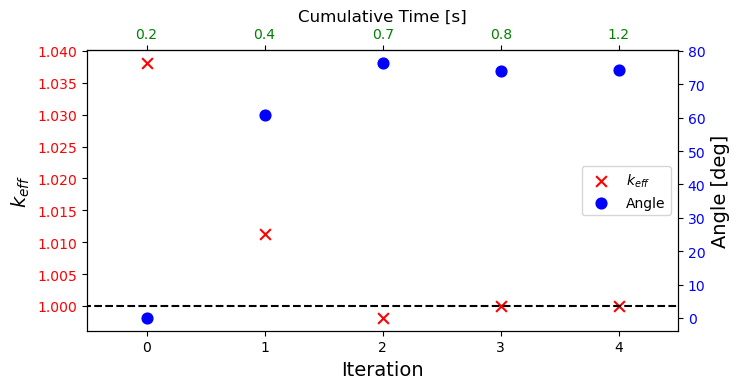
\includegraphics[scale=0.6]{images/angle_keff_power_nomial_example_iteration.png} 
    \caption{$k_{eff}$ and CDs angle as a function of criticality search algorithm iterations (P=2 MW, nominal). The upper x-axis shows the cumulative time of each iteration.}
    \label{fig:angle_keff_evolution_iteration_nominal_power_example}
\end{figure}

In this case, only five iterations are required to reach the criticality state. 
Each iteration is the output of the nested cycle shown in the flow chart in \cref{fig:crit_search_unified_loop}. Consequently, each iteration requires more than one FM solution to converge on the fuel temperature distribution (generally the convergence of the inner cycle is reached after 3-4 iterations).
In total, the converged configuration is obtained after 1.2 s using a single core.   

An equivalent process using a Monte Carlo code would have required 2.1 h for each iteration using the available resources (on 30 cores). This estimate is based on the average execution time reported in \cref{subsec:Computational time needed for the FMDB}. Overall, assuming an equal number of iterations, the entire criticality search would have taken 10.5 h, resulting in a speedup of $3.15 \cdot 10^4$. It is important to note that this value does not include the database pre-calculation effort, discussed in \Cref{subsec:Computational time needed for the FMDB}, which only happens once and can be applied for any system configuration within the database validity range.

\subsection{Computational Time Needed by the FMDB}
\label{subsec:Computational time needed for the FMDB}

The entire study was conducted using a 30-core workstation equipped with an Intel® Xeon® Gold 6130 CPU @ 2.1 GHz.  
\Cref{tab:FMDBresources} summarizes the computational resources employed and the time requirements for generating the Fission Matrix Database (FMDB).  
A total of 136 basic FMDB calculations were performed, complemented by 17 RCR reference runs, for a total of 153 individual Monte Carlo criticality calculations, using Serpent 2.  
The overall wall-clock time required to complete the FMDB generation amounted to 324 hours, which corresponds to an average of approximately 63 CPU hours per simulation.  
These values provide an indication of the computational effort required by the proposed methodology and may serve as a reference for future scaling and optimization studies.

\begin{table}[h!]
\centering
\FloatBarrier
\caption{Computational resources and calculation time requirements for the FMDB generation.}
\label{tab:FMDBresources}
\begin{tabular}{ll}
\hline
Number of basic FMDB calculations       & 136                                      \\ \hline
Number of \rtwo{RCR} reference calculations              & 17                                       \\ \hline
Total number of calculations            & 153                                      \\ \hline
FMDB - total computational time         & 324 h                                    \\ \hline
Average computational time - single core & 63 CPUh                                  \\ \hline
CPU type                                & Intel® Xeon® Gold 6130 @ 2.1 GHz          \\ \hline
Number of cores                         & 30                                       \\ \hline
\end{tabular}
\end{table}

\section{Conclusions and Future Perspectives}

The results presented confirm that the Fission Matrix (FM) method, combined with the RCR, provides a reliable estimation of reactivity parameters under a variety of thermal conditions and control elements configurations.

For this study a linear interpolation between FMDB entries was adopted and the necessary database size was selected by increasing the number of entries to achieve a reasonably low error for the criticality eigenvalue, compared to the statistical uncertainty of Monte Carlo calculation. The final database features 136 FMs, corresponding to eight fuel temperatures and seventeen control drum angles, to which the seventeen reference matrices with the imposed temperature gradient have to be added. Each calculation required, on average, 63 CPUh. These calculations were performed on a PC equipped with an Intel® Xeon® Gold 6130 CPU @ 2.1 GHz, utilizing 30 cores. 
 
In the first set of test cases with imposed temperature gradients between the core and reflector (\cref{tab:cases_testing_cases_for_gradient_T2}), significant deviations in $k_{eff}$ were observed when no correction was applied. $\Delta k_{eff}$ reached 415 pcm in the worst configuration, and the relative error of the fission source reached higher values in the cells that directly face the reflector. The application of the correction ratio notably reduced such discrepancies, with RMSE values generally below 1\% and corrected $\Delta k_{eff}$ values of the same order of magnitude as the combined uncertainty of the reference and of the interpolated matrix.

For test Cases 5--7 (\cref{tab:testing_cases_5_6_7}), involving non-uniform temperature distributions, the method maintained good levels of accuracy even for non-realistic high temperature gradients inside the system (Cases 5 and 6). The results suggest that the proposed correction approach is applicable even when the temperature varies spatially inside the core. Case 7, which uses a temperature distribution that is proportional to the fission source, yielded low errors across all evaluated metrics, indicating that the method remains effective under realistic operating conditions.

The criticality search algorithm based on the FM approach was also tested at different power levels (Cases 8-11, \cref{tab:testing_cases_8_9_10_11}). The computed control drum angles produced reactivity results close to the target critical condition, with RMSE values under 1\% and maximum errors up to 2.2\%. These outcomes suggest that the method can be used to support the estimation of critical configurations under varying thermal conditions with limited deviation from the reference Serpent 2 results. 

In future works, the proposed method will be extended by showing the effect of using different interpolation methods and, in particular, the advantage of using machine learning techniques, like Neural Networks, to improve the matrix interpolation and/or to enable the possibility to use a lower amount of calculation for building up the starting database. 
Moreover, transient analyses will be studied by computing the static reactivity at each time step of the point kinetics equations using the Fission Matrix approach, as suggested in \cite{Dalinger2024}, or by using a transient fission matrix \cite{Mascolino2024}. This would enable the evaluation of reactivity changes at each time step based on a 3D transport-informed model. Furthermore, to account for different transient scenarios, the method could be refined to consider the rotation of only a subset of CDs, rather than all of them simultaneously \cite{Mascolino2022}. For longer time-scale transients and for criticality search throughout operation of the reactor, the effects of fuel burnup and xenon concentration will also be considered \cite{Roskoff2018,Pungercic}.

\section*{Acknowledgements}
The authors acknowledge that the research activity of the PhD project is sponsored by the Italian funding plan ``Piano Nazionale Ripresa e Resilienza'' (PNRR) and by Westinghouse Electric Company. \\ The manuscript has been contributed by UChicago Argonne, LLC, Operator of ANL. ANL, a DOE Office of Science laboratory, is operated under contract number DE-AC02-06CH11357. \\
This research activity has been carried over during the author’s internship period at Argonne National Laboratory.
\bibliographystyle{elsarticle-num-names} 
\bibliography{bibliography}

\end{document}


